%% LyX 2.3.3 created this file.  For more info, see http://www.lyx.org/.
%% Do not edit unless you really know what you are doing.
\documentclass[onluarkali,turkce,yukseklisans,bez,deprem]{itutezLyX}
\usepackage[T1]{fontenc}
\usepackage[utf8]{inputenc}
\setcounter{secnumdepth}{3}
\setcounter{tocdepth}{3}
\usepackage{amsmath}
\usepackage{graphicx}

\makeatletter

%%%%%%%%%%%%%%%%%%%%%%%%%%%%%% LyX specific LaTeX commands.
%% Because html converters don't know tabularnewline
\providecommand{\tabularnewline}{\\}

%%%%%%%%%%%%%%%%%%%%%%%%%%%%%% User specified LaTeX commands.
% ---------------------------------------------------------------- %
%                     LATEX Tez Sablonu                            %
%                                                                  %
%                       Surum 1.5.1                                %
% ---------------------------------------------------------------- %

% ---------------------------------------------------------------- %
% ITU Bilisim Enstitusu tarafindan hazirlanmistir.                 %
%                                                                  %
% İTÜ Ayazağa Kampüsü, Bilişim Enstitüsü Binası                    %
% Maslak-34469, İstanbul                                           %
% http://www.be.itu.edu.tr                                         %
% ---------------------------------------------------------------- %

% ---------------------------------------------------------------- %
% documentclass kullanim argumanlari:                              %
% [onluarkali,tekyonlu],[turkce,ingilizce],[yukseklisans,doktora], %
% [bez,karton],[bilisim,fenbilimleri,sosyalbilimler,avrasya,enerji]%
% Ornek kullanim: \documentclass[onluarkali,ingilizce,yukseklisans,%
% karton,fenbilimleri]{itutezLyX}                                     %
% Baska Ornek kullanim: \documentclass[tekyonlu,ingilizce,         %
% yukseklisans,bez,bilisim]{itutezLyX}                                %
% ---------------------------------------------------------------- %
% \documentclass[onluarkali,turkce,yukseklisans,bez,fenbilimleri]{itutezLyX}
% documentclass LyX içerisinde tanımlanmıştır. BE. 2018-10-05
% ---------------------------------------------------------------- %
% Komutlarda buyuk ve kucuk harf ayrimina ozen gostermek           %
% gereklidir. Ornegin argumanin {\"O\u{g}\-ren\-ci Ad{\i}}{SOYADI} %
% yapisinda olmasi demek, adlarda ilk harflerin buyuk ve           %
% digerlerinin kucuk, soyadinda ise butun harflerin buyuk olmasi   %
% gerektigi anlamina gelmektedir.                                  %
% ---------------------------------------------------------------- %

% ---------------------------------------------------------------- %
% Sadece Ad SOYAD yazilmalidir. Unvan yazilmamalidir.              %
% ---------------------------------------------------------------- %
\yazar{Ahmet}{KARABACAK} 
\ogrencino{802161201}

% ---------------------------------------------------------------- %
% Kullanmayacaginiz yapilarin ayirac aralarini bos birakiniz.      %
% Ornek: \unvan{}                                                  %
% ---------------------------------------------------------------- %
\unvan{İnşaat Mühendisi}
 
% ---------------------------------------------------------------- %
% Asagidaki yapilarda birinci oge Turkce, ikinci oge Ingilizce     %
% yapiyi olusturmak icindir.                                       %
% ---------------------------------------------------------------- %

% ---------------------------------------------------------------- %
% Sozcuklerin ilk harfleri buyuk, diger harfler kucuk yazilacak.   %
% ---------------------------------------------------------------- %
\anabilimdali{Deprem M\"uhendisli\u{g}i Anabilim Dal{\i}}{Department of Earthquake Engineering}
\programi{Deprem M\"uhendisli\u{g}i Program{\i}}{Earthquake Engineering Programme}

% ---------------------------------------------------------------- %
% Beyaz cilt hazirlarken bolume verildigi tarih esas alinir.       %
% Bez (mavi-siyah) ciltte ise tezin savunuldugu tarih ay yil       %
% olarak yazilir.                                                  %
% ---------------------------------------------------------------- %
\tarih{KASIM 2019}{NOVEMBER 2019}
\tarihKucuk{Kas{\i}m 2019}{November 2019}

% ---------------------------------------------------------------- %
% Danisman, baslik ve tez tarihi bilgileri icin asagidaki yapi     %
% kullanilmaktadir.                                                %
% ---------------------------------------------------------------- %

% ---------------------------------------------------------------- %
% Danisman bilgisi, beyaz kapakli tezde ilk sayfada var. Bez       %
% (mavi-siyah) ciltte yok. Neden? Cunku ic kapakta gececek.        %                  
% ---------------------------------------------------------------- %
\tezyoneticisi{Doç. Dr. Barlas Özden ÇAĞLAYAN}{\.Istanbul Teknik \"Universitesi}   

\baslik{OPENSEES VE SEISMOSTRUCT PROGRAMLARININ}{DOĞRUSAL OLMAYAN DEPREM ANALİZLERİ İÇİN}{KARŞILAŞTIRILMASI}{}
\title{COMPARISON OF OPENSEES AND SEISMOSTRUCT PROGRAMS}{FOR NONLINEAR EARTHQUAKE ANALYSIS}{}

% ---------------------------------------------------------------- %
% Bu tarih beyaz kapakli ilk tezin bolume verildigi tarihtir.      %
% ---------------------------------------------------------------- %
\tezvermetarih{15 Kasım 2019}{KASIM 2019} 

\tezsavunmatarih{10 Aralık 2019}{ARALIK 2019}

% ---------------------------------------------------------------- %
% Esdanisman ve juri bilgileri asagidadir. Kullanmayacaginiz satiri%
% tumuyle silmeyiniz. Argumanini bos birakiniz.                    %
% Ornek: \esdanismani{}{}                                          %
% ---------------------------------------------------------------- %
\esdanismani{Dr. Kerem PEKER}{Erdemli Proje Müşavirlik}   

\juriBir{Prof. Dr. Elişan Filiz PİROĞLU}{\.Istanbul Teknik \"Universitesi}

\juriIki{Prof. Dr. Bülent AKBAŞ}{Gebze Teknik \"Universitesi}  

\juriUc{}{}

\juriDort{}{}

\juriBes{}{}

\usepackage{array}
\usepackage{color}
\usepackage{times}
\usepackage{amssymb,amsmath,mathptmx,amsbsy,bm}
\usepackage{caption}            %%
%\usepackage{floatflt}
%\usepackage[dvipdfm]{graphicx}
\usepackage{graphicx}
\usepackage{wrapfig}
\usepackage{epsfig}
\usepackage{enumerate}
\usepackage{rotating}
\usepackage{multirow}
\usepackage{subfigure}
\usepackage{colortbl}
\usepackage{pstricks}
\usepackage{pst-plot}
\usepackage{cite}%
\usepackage{latexsym}           % 
%\usepackage{subeqn}
\usepackage{rotating}
%\usepackage{amssymb}
%\usepackage{hyperref}
%\usepackage{url}
\usepackage{fixltx2e} % Bu paketi sembollerde text ler için subscript yazmakta yardımcı olması için ekliyoruz.

%Bold Equation Number, Unbold Reference
%\makeatletter
%\def\tagform@#1{\maketag@@@{\bfseries(\ignorespaces#1\unskip\@@italiccorr)}}
%\renewcommand{\eqref}[1]{\textup{{\normalfont(\ref{#1}}\normalfont)}}
%\makeatother

%\renewcommand{\theequation}{{\bf\arabic{chapter}.\arabic{equation}}}
%%%%\renewcommand{\thefootnote}{\hskip \arabic{footnote}}

% \def\be{\begin{equation}} %
% \def\ee{\end{equation}}%
% \def\beq{\begin{eqnarray}}%
% \def\eeq{\end{eqnarray}}%
% \def\bse{\begin{subequations}}%
% \def\ese{\end{subequations}}%
% \def\nonu{\nonumber}%
% \def\psibar{\overline{\psi}} %
% \def\Delslash{\partial\!\!\!\!\!/}%
% \def\Gslash{G\!\!\!\!\!/}%
% \def\Lmbdslash{\lambda\!\!\!\!\!/}%
% \def\Jslash{J\!\!\!\!\!/}%
% \def\pslash{p\!\!\!\!/}%
% \def\qslash{q\!\!\!\!/}%
% \def\kslash{k\!\!\!\!/}%
% \def\[{\left[}
% \def\]{\right]}
% \def\({\left(}
% \def\){\right)}

% \def\Lag{{\cal L}}    % 
% \def\D{{\cal D}}      % 
% \def\H{{\cal H}}      % 
% \def\Z{{\cal Z}}      % 
% \def\S{{\textbf{S}}}  % 
% \def\d{{\rm d}}%
% \def\dt{{\rm{dt}}}%
% \def\Tr{{\rm{Tr}}}%
% \def\gm{\gamma^{\mu}}
% \def\ga{\gamma^{\alpha}}
% \def\gb{\gamma^{\beta}}
% \def\gn{\gamma^{\nu}}
% \def\gs{\gamma^{\sigma}}
% \def\gl{\gamma^{\lambda}}
% \def\gr{\gamma^{\rho}}
% \def\gd{\gamma^{\delta}}


% ---------------------------------------------------------------- %
% Ithaf sayfasinda bulunacak tumceler icin kullanilabilecek        %
% yapi asagidadir. Ithaf sayfasi bulunmayacaksa argumani(ayiraclar %
% arasini) bos birakiniz.                                          %
% ---------------------------------------------------------------- %
\ithaf{Ecem Şengüle,}

% ---------------------------------------------------------------- %
% Asagida belirtilen tex uzantili dosyalarin icerigi               %
% olusturulmalidir.                                                %
% ---------------------------------------------------------------- %

\onsoz{	Bu tez çalışması süresince samimiyetini ve hoşgörüsünü benden esirgemeyen,
	bilgisi ile her zaman istifade ettiğim danışman hocam Doç. Dr. Barlas
	Özden ÇAĞLAYAN’a, mesleki eğitim sürecimin başından beri vizyonu ile
	yolumu aydınlatan, üstadım ve eş danışmanım Dr. Müh. Kerem PEKER’e
	sonsuz teşekkür ederim.
	
	Çok kıymetli görüşleri ve deneyimlerini benimle paylaşan, İnş. Yük.
	Müh. Ahmet Kaptan’a ve İnş. Yük. Müh. Ahmet Metin YILDIRIM’a teşekkürü
	bir borç bilirim.
	
	Bu süreçte desteğini esirgemeyen motivasyon kaynağım İnş. Yük. Müh.
	Ecem Şengül’e çok teşekkür ederim. 
	
	Tezin hazırlanması aşamasında yardımları için Dr. Ögr. Üyesi Barış
	ERKUŞ’a ve mesai arkadaşım İnş. Yük. Müh. Mehmet Gezer’e teşekkür
	ederim.
	
	Ayrıca bu yüksek lisans tezi 42127 numaralı İTÜ-Bilimsel Araştırma
	Projesi kapsamında kabul görmüştür, destekleri için İstanbul Teknik
	Üniversitesi’ne teşekkürlerimi sunarım.
	
	Hayatım boyunca bana her zaman güvenen, koşulsuz destekleyen ve her
	daim yanımda hissettiğim aileme, annem Kadriye KARABACAK, babam İbrahim
	KARABACAK’a ve kardeşlerime teşekkür ederim.}
\kisaltmalistesi{\hspace{-3mm} %
\begin{tabular}{p{2cm}l}
\textbf{AASHTO} & \textbf{:} American Association of State Highway and Transportation
Officials \tabularnewline
\textbf{ASCE} & \textbf{:} American Society of Civil Engineers \tabularnewline
\textbf{CALTRANS}  & \textbf{:} California Department of Transportation \tabularnewline
\textbf{DBYBHY} & \textbf{:} Deprem Bölgelerinde Yapılacak Binalar Hakkında Yönetmelik \tabularnewline
\textbf{FEMA}  & \textbf{:} Federal Emergency Management Agency \tabularnewline
\textbf{PEER}  & \textbf{:} Pacific Earthquake Engineering Research Center \tabularnewline
\textbf{SEI} & \textbf{:} Structural Engineering Institute \tabularnewline
\textbf{TBDY}  & \textbf{:} Türkiye Bina Deprem Yönetmeliği \tabularnewline
\textbf{New} & \textbf{:} New Explanation\tabularnewline
\end{tabular}
}
\sembollistesi{\global\long\def\tabcolsep{1pt}%
\renewcommand\arraystretch{1.1}%

\noindent \hspace{-3mm} %
\begin{longtable}{>{\raggedright}p{1cm}l>{\raggedright}p{13.4cm}}
$a_{0}$ & : & Rayleigh sönüm matrisi için kütle matrisi çarpanı\tabularnewline
$a_{1}$ & : & Rayleigh sönüm matrisi için rijitlik matrisi çarpanı\tabularnewline
$a_{1}$ & : & Menegotto-Pinto modelinde Baushinger malzeme sabitleri\tabularnewline
$a_{2}$ & : & Menegotto-Pinto modelinde Baushinger malzeme sabitleri\tabularnewline
$A_{\text{co}}$ & : & Sheik ve Uzumeri modelinde beton çekirdek alanı\tabularnewline
$A_{\text{s}}$ & : & Sheik-Uzumeri ve Saatçioğlu-Ravzi modellerinde enine donatı alanı\tabularnewline
$A_{\text{sx}}$ & : & Mander modelindende $x$-doğrultusunda uzanan toplam enine donatı
kesit alanı\tabularnewline
$A_{\text{sy}}$ & : & Mander modelindende $y$-doğrultusunda uzanan toplam enine donatı
kesit alanı\tabularnewline
$b$ & : & Mander modelindende enine donatı merkezlerinden ölçülen çekirdek betonunun
$x$-yönüne paralel boyutu\tabularnewline
$b$ & : & Sheik-Uzumeri modelinde çekirdek betonun kenar uzunluğu\tabularnewline
$b_{\text{c}}$ & : & Saatçioğlu-Ravzi modelindende kare kesit çekirdek betonu uzunluğu\tabularnewline
$b_{\text{cx}}$ & : & Saatçioğlu- Ravzi modelindende çekirdek betonun $x$-doğrultusu uzunluğu\tabularnewline
$b_{\text{cy}}$ & : & Saatçioğlu-Ravzi modelindende çekirdek betonun $y$-doğrultusu uzunluğu\tabularnewline
$\mathbf{b}$ & : & Fiber modelde kuvvet interpolasyon fonksiyonu\tabularnewline
$C$ & : & Sheik ve Uzumeri modelinde düşey donatıların eksenleri arasındaki
uzaklık\tabularnewline
$\mathbf{C}$ & : & Sönüm matrisi\tabularnewline
$\mathbf{d}$ & : & Şekil değiştirme matrisi\tabularnewline
$\mathbf{D}$ & : & İç kuvvet matrisi\tabularnewline
$E_{\mathrm{c}}$ & : & Betonun elastisite modülü \tabularnewline
$E_{\text{s}}$ & : & Donatı çeliğinin elastisite modülü\tabularnewline
$E_{\text{sh}}$ & : & Mander çelik modelindende pekleşme modülü\tabularnewline
$F_{\text{y}}$ & : & Akma gerilmesi\tabularnewline
$E_{\text{t}}$ & : & Mander çelik modelindende tanjant elastisite modülü\tabularnewline
$f_{\text{c}}$ & : & Hognestod, Mander ve Kent-Park modellerinde beton basınç gerilmesi\tabularnewline
$f_{\text{c}}^{''}$ & : & Hognestod modelindende betonun maksimum basınç dayanımı\tabularnewline
$f_{\text{c}}^{'}$ & : & Hognestod modelindende beton karakteristik basınç dayanımı\tabularnewline
$\mathit{f}_{\text{c}}'$ & : & Sheik ve Uzumeri modelindende sargılı beton basınç dayanımı\tabularnewline
$f_{\text{cc}}^{'}$ & : & Sheik ve Uzumeri modelindende beton basınç gerilmesi\tabularnewline
$f_{\text{cc}}^{'}$ & : & Mander modelindende sargılı betonda kırılma anında birim şekil değiştirmesi\tabularnewline
$f_{\text{co}}^{'}$ & : & Mander modelindende sargısız betonun basınç dayanımı \tabularnewline
$f_{\text{l}}^{'}$ & : & Mander modelindende ortalama etkili sargılama basıncı\tabularnewline
$f_{\text{lx}}^{'}$ & : & Mander modelindende $x$-doğrultusundaki etkili sargılama basıncı\tabularnewline
$f_{\text{ly}}^{'}$ & : & Mander modelindende $y$-doğrultusundaki etkili sargılama basıncı\tabularnewline
$f_{\text{yh}}$ & : & Mander modelindende enine donatının akma dayanımı\tabularnewline
$f_{\text{yt}}$ & : & Enine donatının akma dayanımı\tabularnewline
$f_{\text{1e}}$ & : & Saatçioğlu ve Ravzi modelindende ortalama yanal sargı basıncı\tabularnewline
$f_{\text{1ex}}$ & : & Saatçioğlu ve Ravzi modelindende $x$-doğrultusunda oluşan etkili
sargı basıncı\tabularnewline
$f_{\text{1ey}}$ & : & Saatçioğlu ve Ravzi modelindende $y$-doğrultusunda oluşan etkili
sargı basıncı\tabularnewline
$f_{\text{yw}}$ & : & Kent-Park modelindende enine donatının akma dayanımı\tabularnewline
$f_{\text{sy}}$ & : & Mander çelik modelindende donatı akma dayanımı\tabularnewline
$f_{\text{su}}$ & : & Mander çelik modelindende donatı nihai dayanımı\tabularnewline
$f_{\text{s}}^{'}$ & : & Sheik ve Uzumeri modelinde enine donatının akma dayanımı\tabularnewline
$\mathbf{f}$ & : & Fleksibilite (esneklik) matrisi\tabularnewline
$\mathbf{F}_{\text{s}}$ & : & Rijitlik tarafından üretilen kuvvet\tabularnewline
$\mathbf{F}_{\text{s},i}^{\text{denge}}$ & : & Dengelenmemiş kuvvet\tabularnewline
$\mathbf{F}_{\text{s},i}^{\text{kabul}}$ & : & Başlangıç rijitliğine bağlı olarak varsayılan kuvvet\tabularnewline
$\mathbf{F}_{\text{s},i}^{\text{içkuv}}$ & : & Bünye fonksiyonlarından elde edilen iç kuvvet\tabularnewline
$h^{'}$ & : & Kent-Park modelinde sargılı beton kısmının etriye dışından etriye
dışına genişliği\tabularnewline
$h$ & : & Mander modelinde enine donatı merkezlerinden ölçülen çekirdek betonunun
$y$-yönüne paralel boyutu\tabularnewline
$\text{k}_{\text{e}}$ & : & Mander modelinde sargılamanın etkinliği ile ilgili katsayı\tabularnewline
$K_{\text{s}}$ & : & Pekleşme rijitliği \tabularnewline
$K_{\text{e}}$ & : & Başlangıç rijitliği\tabularnewline
$\mathbf{K}_{\text{T},i}^{j}$ & : & $i.$ zaman adımı ve $j.$ iterasyon için rijitlik matrisi \tabularnewline
$\mathbf{K}$ & : & Eleman rijitlik matrisi\tabularnewline
$M_{y}$ & : & $y$-eksenine göre eğilme momenti\tabularnewline
$M_{z}$ & : & $z$-eksenine göre eğilme momenti\tabularnewline
$\mathbf{M}$ & : & Kütle matrisi\tabularnewline
\end{longtable}

\noindent 
\global\long\def\tabcolsep{6pt}%
\renewcommand\arraystretch{1.0}%
}
\ozet{Depremselliğin yüksek olduğu bölgelerde bulunan yapıların kuvvetli
yer hareketleri sebebiyle hasar almalarını engellemek amacıyla sismik
yalıtım sistemleri sıklıkla kullanılmaktadır. Sismik yalıtımlı yapılar
üst yapı, yalıtım düzlemi ve yalıtım birimlerinden oluşmaktadır. Bu
sistemler çoğunlukla izolatörlerin üzerinde göreli olarak rijit hareket
ettiği kabul edilen konut, veri merkezi binası, hastane yapıları,
sıvı tankı ve açık deniz petrol platformu gibi tek yapılardır. Birbirinden
bağımsız sismik yalıtımlı yapıların birlikte kullanılmaları durumunda
çözülmesi gereken mimari detaylar karmaşık ve pahalı olmaktadır. Bu
sebeple pratikte birbirinden bağımsız bina tipi yapılar ortak yalıtım
düzleminde tasarlanmaktadır. Özellikle Türkiye'de son yıllarda yapılan
hastane yapıları bu tanıma uymaktadır.

Geçmişte yapılan çalışmalar neticesinde belirlenen doğrusal tasarım
yöntemleri, sismik yalıtımlı yapıları tek veya çok serbestlik dereceli
bir yapıdan oluşan sistemler olarak değerlendirmektedir. Bu nedenle
yönetmeliklerde yer alan tasarım prosedürleri bağımsız yalıtım düzleminde
bulunan sismik yapılar hazırlanmıştır. Ortak yalıtım düzleminde bulunan
sismik yalıtımlı yapılar için ise yönetmeliklerde tasarım kriteri
bulunmamaktadır. Pratikte ortak yalıtım düzleminde tasarlanmış yapıların
her biri bağımsız yalıtım düzleminde analiz edilerek boyutlandırılmaktadır.
Bu sebeple izolatörlerin histeretik davranışlarından kaynaklanan yüksek
mod etkileri dolayısıyla yapıların dinamik etkileşimi değerlendirilememektedir.

Bu çalışmanın amacı ortak yalıtım düzleminde bulunan iki yapı için
kapsamlı parametrik inceleme yapılarak üst yapıların dinamik etkileşimi
sebebiyle oluşan taban kesme kuvvetlerindeki amplifikasyonun irdelenmesidir.

Çalışma kapsamında ortak yalıtım düzlemine sahip iki yapının dinamik
etkileşimi, parametrik olarak değişen sistemler üzerinden incelenmiştir.
Ayrıca ortak yalıtım düzleminde bulunan üç ve dört yapılı sistemler
için örnek çözümler yapılmıştır. Burada üst yapı kat sayısı, yalıtım
birimleri eşdeğer periyot ve eşdeğer sönüm değerleri birer parametre
olarak ele alınmıştır. Ortak yalıtım düzleminde bulunan iki yapı kat
sayısının birden ona değiştiği durumlar için analizler yapılmıştır.
Tüm analizler yalıtım birimlerinin 1.5, 2.5 ve 4.0sn eşdeğer periyot
ve \%10, \%20 ve \%30 eşdeğer sönüm değerleri için tekrarlanmıştır.
Yalıtım birimlerinin histeretik özellikleri, değişen üst yapı kütlesine
karşılık doğrusal olmayan analizler sonucunda sabit eşdeğer periyot
ve eşdeğer sönüm değerlerini elde edebilmek amacıyla normalize edilmiştir.
Bu işlem istenilen eşdeğer periyot değerine karşılık gelen rijitlik
ve eşdeğer sönüm değerleri ile yapılan doğrusal zaman tanım analizlerinden
elde edilen yalıtım birimi yer değiştirmelerine karşılık akma sonrası
rijitlik ve karakteristik dayanımın belirlenmesi ile gerçekleştirilmektedir.

Analizler yalnızca yapıların ortak yalıtım düzleminde bulunduğu doğrultu
için yapılmıştır. Diğer yöndeki etkiler ve yalıtım birimlerinin iki
yönlü etkileşimi göz ardı edilmiştir. Üst yapıların kat kütle ve kat
rijitlikleri tüm analizler için sabit alınmıştır. Yalıtım düzlemi
kütlesi ise her yapı için sabit olup ortak yalıtım düzleminde bulunan
yapı sayısı çarpılarak hesaplanmıştır. Yalnızca kesme yaylarının dikkate
alındığı modellerde üst yapılar çok serbestlik dereceli ve doğrusal
elastik olarak tanımlanmıştır. Yalıtım birimlerinin doğrusal olmayan
davranışları ise çift doğrulu eleman ile temsil edilmektedir. Yalıtım
birimlerinde yalnızca doğrusal olmayan davranıştan kaynaklanan histeretik
sönüm kullanılmıştır. Analizlerde kullanılan deprem kayıtları, 50
yılda aşılma olasılığı \%2 olan deprem yer hareketi düzeyine göre
oluşturulan tasarım spektrumuna uygun olarak eşleştirilmiştir.

Tüm analizler tez kapsamında geliştirilen, bağımsız ve ortak yalıtım
düzleminde bulunan sismik yalıtımlı yapıların doğrusal olmayan analizlerinin
parametrik olarak çözülebilmesine imkan sağlayan MSBIS programı yardımıyla
gerçekleştirilmiştir. Geliştirilen programın doğruluğu, genel kabul
görmüş yapısal analiz programı olan SAP2000 ile karşılaştırılarak
gösterilmiştir.

Yer ivmeleri etkisinde doğrusal olmayan dinamik analizler yapılarak
birinci yapıda meydana gelen kat kesme kuvvetleri, kat ivmeleri ve
göreli kat ötelemeleri ikinci yapının değişen açısal frekansına ve
yalıtım birimlerinin farklı eşdeğer periyot ve eşdeğer sönüm değerlerine
göre değişimi incelenmiştir. Ayrıca birinci yapının on katlı olması
durumunda ikinci yapının değişen kat sayıları için kat kesme kuvveti
katsayıları değişimi irdelenmiştir. Elde edilen sonuçlar, incelenen
yapıların bağımsız yalıtım düzleminde bulunması durumunda elde edilecek
büyüklüklere göre normalize edilmiştir. Böylece yapıların taban kesme
kuvvetlerindeki amplifikasyon üst yapı açısal frekanslarına, yalıtım
birimi eşdeğer periyot ve eşdeğer sönümüne bağlı olarak tespit edilebilmektedir.
Ortak yalıtım düzleminde bulunan yapıların taban kesme kuvveti katsayıları
elde edilerek sonuçlar yapıların dinamik analizde vektörel olarak
toplanarak elde edilen toplam kesme kuvveti katsayısına göre kıyaslanmıştır.
Tespit edilen bu hata oranı yapıların dinamik etkileşiminin mertebesi
ile doğru orantılı olarak artmaktadır. Buna ek olarak ortak yalıtım
düzleminde bulunan iki yapının gerekli deprem derz mesafeleri, yönetmeliklerde
belirtilen yöntemler ile hesaplanarak doğrusal olmayan dinamik analizlerden
elde edilen sonuçlar ile kıyaslanmıştır.

Çalışma sonucunda, yalıtım birimlerinin histeretik sönümlerinin artması
nedeniyle oluşan yüksek mod etkilerinin ortak yalıtım düzleminde bulunan
yapıların taban kesme kuvveti katsayılarını, göreli kat ötelemelerini
ve en büyük kat ivmelerini önemli ölçüde artırdığı tespit edilmiştir.
Bu artışın, iki yapının açısal frekansların ayrıklaşması ile arttığı
görülmüştür. Dolayısıyla iki yapının da aynı açısal frekansa sahip
olması durumunda elde edilen iç kuvvet ve yer değiştirmeler, yalıtım
birimlerinin aynı eşdeğer periyot ve sönüm değerleri için eşit bulunmaktadır.
Ortak yalıtım düzleminde bulunan iki yapıdan incelenen bir katlı yapının
taban kesme kuvvetleri ikinci yapının değişen kat sayılarına karşılık
bağımsız yalıtım düzleminde bulunması durumuna göre artmaktadır. On
katlı yapının incelendiği durumda ise kat kesme kuvvetleri alt katlarda
artarken üst katlar için azaldığı belirlenmiştir. Ortak yalıtım düzleminde
bulunan üç ve dört yapılı sistemler için yapılan analizler sonucunda
ise incelenen yapıdan farklı açısal frekansa sahip yapı sayısının
artmasıyla taban kesme kuvveti katsayılarının arttığı tespit edilmiştir.
Ayrıca histeretik sönümün artması ile taban kesme kuvvetinin üst yapıya
dağılımında ters üçgen formunun oluştuğu belirlenmiştir.
}
\summary{Rubber bearings are used to prevent vibrations in the buildings and
to allow the bearings to be displaced due to thermal expansion in
the bridges. The first use of rubber bearings in order to protect
constructions against earthquake effects, occurred in Pestalozzi primary
school in Skopje, Yugoslavia in 1969. The same horizontal and vertical
stiffness of the rubber supports applied as a single block caused
the bulge to occur due to the weight of the building on the side surfaces.
The French engineer Eugène Freyssinet, who discovered that the axial
loading capacities of the rubber layers were inversely proportional
to their height, suggested strengthening the rubber layers by adding
thin steel plates in the vertical direction. Here the bond between
the layers is provided due to the friction force. Thanks to the vulcanization
method used to ensure that the thin steel plates and rubber layers
adhere to each other, studies and applications of modern seismic isolators
have begun to increase.

Seismic isolation systems are frequently used to prevent damage to
structures in areas with high seismicity due to strong ground motions.
Base isolated structures consist of superstructure, isolation plane
and base isolators. These systems are single structures such as residential,
data center building, hospital, liquid tank and offshore oil platform
which are assumed to displace relatively rigid over the base isolators.
The architectural details to be solved in the case of using separate
base isolated structures together, are complex and expensive. For
this reason independent superstructures are designed in common isolation
plane. More particularly, constructed hospital buildings in recent
years in Turkey, meets this definition.

Linear design methods, which are determined in consequence of carried
out studies in the past, are consider the base isolated systems as
consist of single or multi degree of freedom systems. Therefore design
procedures in standards are prepared for base isolated structures
with independent isolation plane. There is no design criteria in standards
for dynamic interaction of base isolated structures with common isolation
plane. Each of the base isolated structures which are designed in
common isolation plane are considered in practice as if structures
with independent isolation plane. As a consequence of this assumption
causes the higher mode effect due to the hysteretic behavior of the
isolators and therefore the dynamic interaction of superstructures
to be unevaluated.

Purpose of this study is to determine amplification of the base shear
coefficient due to interaction of superstructures by performing comprehensive
parametric investigation for the two base isolated structures with
common isolation plane.

Within the scope of this study, dynamic interaction of two base isolated
structures with common isolation plane is investigated through the
systems changes parametrically. In addition to this sample analyses
are carried out for three and four base isolated structures with common
isolation plane. In this case, number of story of superstructures,
equivalent period and equivalent damping ratio of base isolators are
considered as parameter. Analyses are carried out for the cases where
the number of story of two base isolated structures with common isolation
plane changes from one to ten. All analyses are repeated for 1.5,
2.5, 4.0s equivalent period and \%10, \%20, \%30 equivalent damping
ratio of base isolators. The hysteretic properties of the base isolators
are normalized to obtain constant equivalent period and equivalent
damping ratios as a result of nonlinear analysis versus varying superstructure
mass. This process is performed by determining the yielded stiffness
and characteristic strength by determining the isolator displacements
obtained from the linear time-history analysis with the stiffness
corresponding intended equivalent period and the equivalent damping
values.

Analyses are carried out only for the direction in which the structures
are located in the common insulation plane. The effects that occur
other directions and the bi-directional interactions of the isolators
are out of scope of this study. Story mass and story stiffnesses of
superstructures are fixed for all analyses. Mass of the isolation
plane is fixed for each structure and is calculated by multiplying
the number of structures in the common isolation plane. Only linear
elastic shear springs are considered in superstructure models which
are defined as multi degree of freedom system. Hysteretic behavior
of isolators are represented by a bilinear element. Only hysteretic
damping which is caused by nonlinear behavior is considered in base
isolators. The ground motion records used in the analyses are matched
in accordance with the design spectrum generated according to earthquake
ground motion level with probability of exceeding \%2 in 50 years.

All analyzes were carried out by means of the MSBIS program, which
was developed within the scope of this study, which allows nonlinear
analysis of base isolated structures with independent and common isolation
plane to be solved parametrically. Numerical solution of equation
of motions is carried out with Newmark-$\beta$ method. Dynamical
balance is provided by Newton-Raphson method doing iteration in every
time step. The accuracy of the developed program is demonstrated by
comparison with SAP2000, the generally accepted structural analysis
program.

Resultant shear forces, story accelerations and story drifts of the
first structure is determined by means of nonlinear time history analyses
according to changing angular frequency of the second structure and
effective period and damping values of base isolators. In addition,
for the case of first structure have ten stories, the variation of
story shear force coefficients for the changing number of story of
the second structure is examined. Results are normalized according
to values which obtain from the inspected base isolated structures
with independent isolation plane. Thus, amplification in base shear
forces of the structures can be determined depending on the angular
frequency of the superstructures, equivalent period and equivalent
damping of base isolator. Base shear force coefficients of the structures
with common isolation plane are obtained and the results are compared
according to the total shear force coefficient obtained by vector
summation in the dynamic analysis. This rate of error is increasing
in direct proportion to the order of the dynamic interaction of the
structures. Additionally necessary joint spacing of two base isolated
structures with common isolation plane is calculated as per related
standard and compared to results obtained from the nonlinear dynamic
analysis.

As a result of this study, it is determined that dynamic interaction
of two base isolated structures with common isolation plane due to
increasing damping ratio of base isolators, causes to increase shear
coefficients, story drifts and maximum story accelerations significantly.
This increment is determined to increase with the separation of the
angular frequencies of the two structures. Therefore, if two structures
have the same angular frequency, the resulting internal forces and
displacements are equal for the same equivalent period and equivalent
damping ratios base isolators. Base shear force of one story structure
inspected from two base isolated structures with common isolation
plane, increase with respect to vary other structure number of story
according to situation that inspected structure with independent isolation
plane. When the ten-story structure is examined, it is determined
that the story shear forces increase in the lower stories and decrease
in the upper stories. As a result of the analyses carried out for
the three and four base isolated structure with common isolation plane,
it is determined that the base shear force coefficients increase with
the increase of the number of buildings having different angular frequency
from the examined structure. Moreover, increasing in hysteretic damping
causes to change lateral distribution of base shear forces to superstructure.
Base shear force of structure is evenly distributed to every story
for an equivalent damping value of \%1, which is assumed to be linear
of the isolators. Nevertheless, base shear force of structure is distributed
in the form of an inverted triangle for increasing damping ratios.
}

%------------------------------------%
% Packages added by BE
\usepackage{hypenTR}
\usepackage{longtable}
%------------------------------------%

%------------------------------------------------------------------%
% Matrisler için bazı ek araçlar                                   %
% Eğer \input olarak girilmiş LyX dosyalarında kullanılacaksa,     %
% bunları o dosyaya kopyalayarak "Instant Preview ile denklemler   %
% görülebilir                                                      %
%                                                                  %
\usepackage{upgreek}
\usepackage{pdfrender}
\newcommand*{\boldgreek}[1]{%
  \textpdfrender{%
    TextRenderingMode=FillStroke,%
    LineWidth=.35pt,%
  }{#1}%
}
%
% BE, 2018-10-05
%------------------------------------------------------------------%

% ---------------------------------------------------------------- %
% Custom commands
% ---------------------------------------------------------------- %
%\renewcommand*\arraystretch{1.5}   % To increase the row height of tables
%Heceleme için hyphenpenalty değerini küçültebilirsiniz. 
%Değer küçüldükçe hecelemek isteyecek, değer büyükdükçe hecelemekten kaçacaktır.
%This block moved to the LaTeX file for convenience
\hyphenpenalty=10000
\exhyphenpenalty=10000
\widowpenalty=10000
\clubpenalty=10000

\makeatother

\begin{document}

\chapter{GİRİŞ}

\label{CH1}

Deprem bölgelerinde yapılacak binalarda yaygın olarak kullanılan kuvvet
esaslı tasarıma göre, yapının karşılaşması beklenen en büyük deprem
kuvveti altında göreli olarak büyük yer değiştirmeler yapması, yapısal
taşıyıcı elemanlarda hasar oluşması ve dolayısıyla deprem enerjisinin
büyük bir kısmının kalıcı şekil değiştirmeler ile sönümlenmesi beklenir.
Yapının önem derecesine bağlı olarak depremde daha az hasar almasını
sağlamak amacıyla göreli kat ötelemelerinin sınırlanması gerekmektedir.
Bu durum, yapının rijitliğini artırarak katlarda daha büyük ivmelerin
oluşmasına ve buna bağlı olarak yapısal olmayan elemanlarda daha büyük
kuvvetlerin oluşmasına sebep olmaktadır. Kat ivmelerinin azaltılması
ise yapı rijitliğinin düşürülmesi ile mümkündür. Ancak bu durumda
göreli kat ötelemeleri ve yapısal hasarlar artmaktadır. Yapıların
depremden korunmasının bir yolu, zemin ile yapı temeli arasında, yatay
rijitliği yapıya oranla düşük bir katman oluşturmaktır.

Yapılarda kuvvetli yer hareketleri sebebiyle oluşan hasarları engellemek
amacıyla birçok yöntem üzerine çalışmalar yapılmıştır. Touaillon 1870
yılında, ABD patent ofisine yaptığı başvuruda, temel ve binaya sabitlenen
konkav metal plakaların arasında bulunan küreler sayesinde deprem
sebebiyle yapıların yıkılmasının önleneceğini söylemektedir \cite{Touaillon1870}.
Benzer bir yalıtım sistemi ise Bechtold tarafından 1907 yılında patent
başvurusu yapılan, binaların altına yerleştirilen rijit taban plakasının
bazalt, gnays veya granitten yapılacak küreler üzerinde kayan bir
sistem önerisidir \cite{Bechtold1907}. Dr. Calantarines ise yapı
temelinin ince kum, mika veya talk üzerinde kayabildiği bir ``serbest
mesnet'' fikri ile 1909 yılında İngiltere patent ofisine başvurmuştur
\cite{calantarients1909improvements}.

Yeni yöntemlerin araştırılmasının yanında üst katlarda önemli hasarların
oluşmasını engellemek amacıyla yumuşak ilk kata sahip yapılar da depreme
etkileri altında incelenmiştir. Chopra ve diğerleri tarafından yapılan
çalışmada ilk katı yumuşak kata sahip sekiz katlı bir binanın, deprem
etkileri altında üst katlarında hasar oluşmasını engellemek amacıyla
ilk katın akma koşulları incelenmiştir \cite{doi:10.1002/eqe.4290010405}.

Kauçuk mesnetler, binalarda titreşimleri engellemek ve köprülerde
ise ısıl genleşmeler sebebiyle mesnetlerin yer değiştirebilmelerini
sağlamak amacıyla kullanılmıştır. Yapıların deprem etkilerinden korunmaları
amacıyla ilk kullanımı 1969 yılında Yugoslavya'nın Skopje ilinde bulunan
Pestalozzi ilkokulunda gerçekleşmiştir. Tek bir blok olarak uygulanan
kauçuk mesnetlerin yatay ve düşey rijitliklerinin aynı olması, yan
yüzeylerde binanın ağırlığından dolayı şişkinlik oluşmasına neden
olmuştur. Kauçuk katmanların eksenel taşıma kapasitelerinin yükseklikleri
ile ters orantılı olduğunu tespit eden Fransız mühendis Eugène Freyssinet,
kauçuk katmanların aralarına eksenel kuvvete dik doğrultuda ince çelik
plakalar ilave ederek güçlendirmeyi önermiştir. Burada katmanlar arasındaki
bağ sürtünme kuvveti sebebiyle sağlanmaktadır. İnce çelik plakalar
ile kauçuk katmanların birbirlerine yapışmalarını sağlamak amacıyla
kullanılan vulkanizasyon yöntemi sayesinde modern haline kavuşan sismik
izolatörler ile ilgili yapılan çalışmalar ve uygulama örnekleri artmaya
başlamıştır. Kelly tarafından yapılan çalışmada 1900-1984 yılları
arasında sismik yalıtım çalışmaları özetlenerek alfabetik ve kronolojik
bibliyografya sunulmuştur \cite{KELLY1986202}.

Robinson ve Tucker tarafından gerçekleştirilen çalışmada, Şekil \ref{fig:LRBIsolator}'de
gösterilen çelik plakalar ile güçlendirilmiş kauçuk izolatörün merkezine
kurşun silindir yerleştirilerek tekrarlı yatay yükler etkisindeki
davranışı incelenmiştir \cite{RobinsonTucker1977}. Çelik ve kauçuk
ile sargılı olan kurşun silindirde tamamen kayma deformasyonları meydana
gelmektedir. Çalışmada, günümüzde yaygın olarak kullanılan bu sistemin
sahip olduğu histeretik sönüm kapasitesi, kurşun çekirdeğin eksenel
dayanımı ve geri çağırım kuvveti gibi faydaları belirtilerek büyük
deprem etkileri ve küçük rüzgar yüklerinde yeterli performans sergileyeceği
vurgulanmıştır.
\begin{figure}[h!]
\centering{}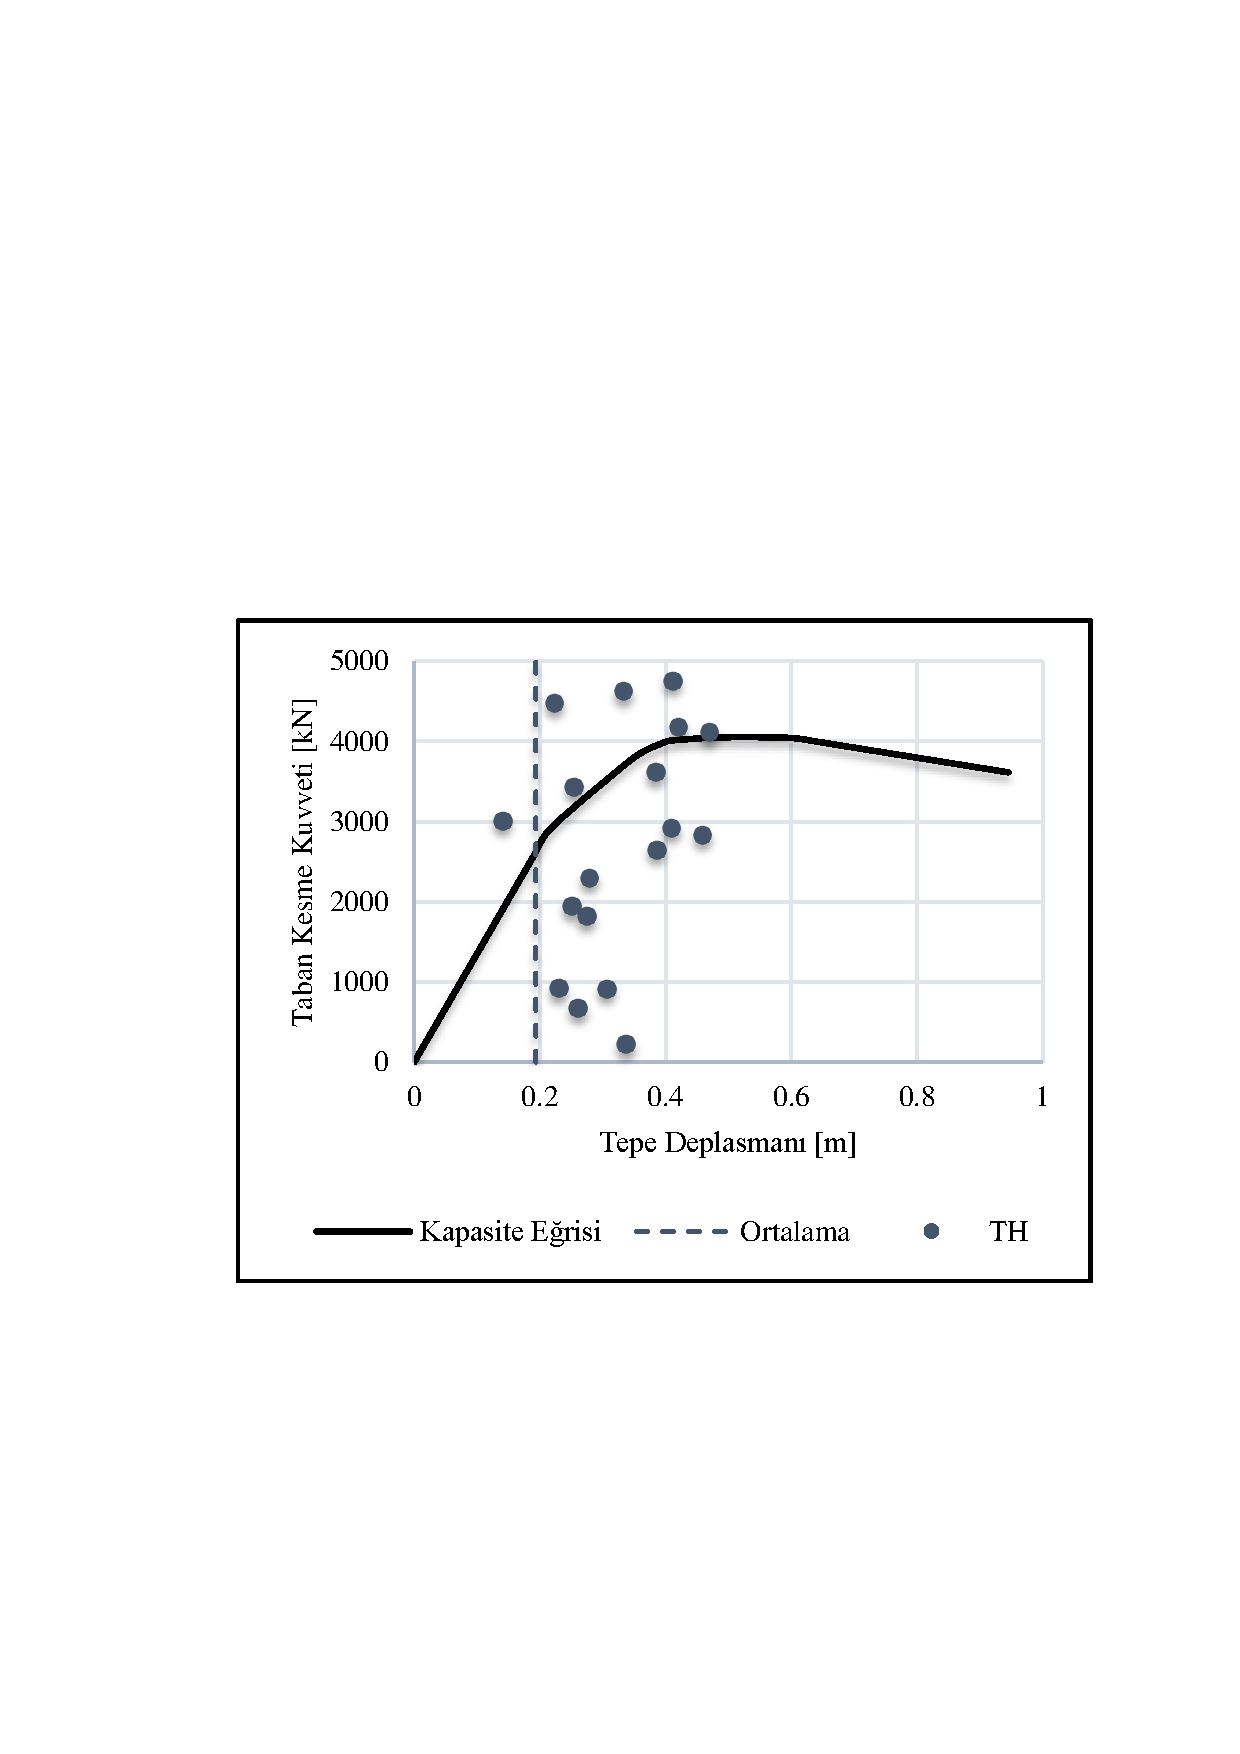
\includegraphics[width=6.5cm,height=6cm]{TikZ/Grafik_1}\hspace{1cm}
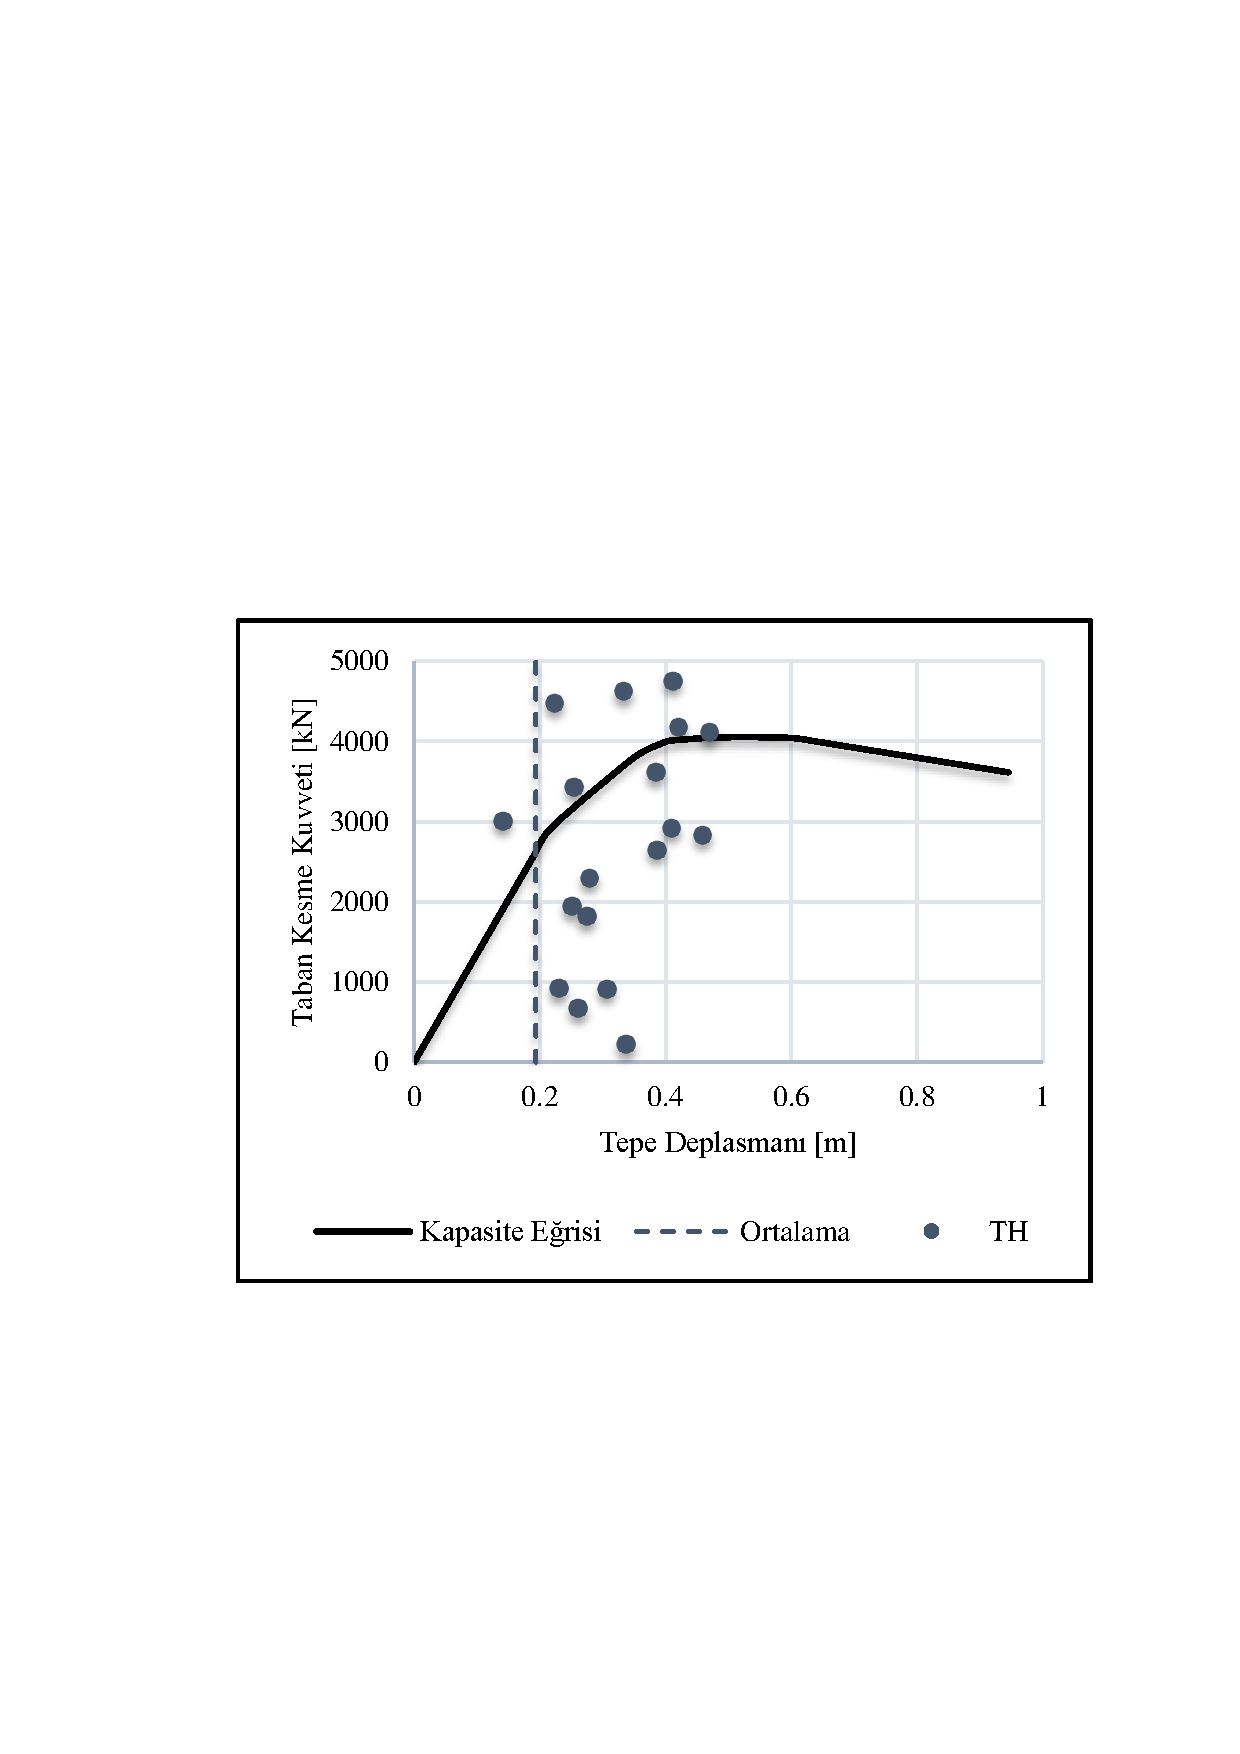
\includegraphics[width=6.5cm,height=6cm]{TikZ/Grafik_1}\caption{\label{fig:LRBIsolator} Kurşun çekirdekli kauçuk izolatör.}
\end{figure}

Yapıların mesnetleri üzerinde sarkaç gibi hareket etmelerini sağlayan
sismik yalıtım yöntemi Zayas ve diğerleri tarafından 1990 yılında
yapılan çalışmalar neticesinde önerilmiştir \cite{doi:10.1193/1.1585573}.
Şekil \ref{fig:FPIsolator}'de kesiti verilen sürtünmeli sarkaç tipi
izolatörlerin yalıtım periyotları konkav yüzeyin yarıçapı ile belirlenmektedir.
Deprem enerjisinin sönümlendiği histeretik davranış, yüzeylerde oluşan
sürtünme kuvvetleri nedeniyle oluşmaktadır. Sistemin sarkaç hareketine
başlaması, sürtünme kuvvetlerinin aşılmasıyla mümkün olmaktadır. Bu
nedenle yapının rüzgar yükleri altında yalıtım birimlerinden beklenen
rijitlik elde edilmiş olmaktadır. Sürtünmeli sarkaç tipi izolatörlerin
malzeme belirsizliklerinden en az düzeyde etkilenmesi, sismik yalıtımlı
yapıların deprem etkileri altındaki davranışlarının öngörülebilir
olmasını sağlamaktadır. Ayrıca yapılan testlere göre büyük deplasmanlarda
eksenel taşıma kapasitesinde düşme veya stabilite kaybı olmadığı ve
histeretik çevrimler ile dayanım azalmasının oluşmadığı görülmüştür.
\begin{figure}[h!]
\centering{}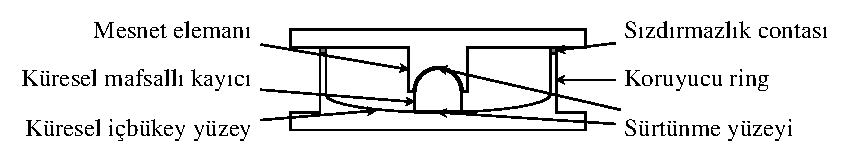
\includegraphics{TikZ/FPIsolator} \caption{\label{fig:FPIsolator}Sürtünmeli sarkaç tipi izolatör.}
 
\end{figure}

Sismik izolasyon, dünyada depremselliği yüksek olan bölgelerde yoğun
olarak kullanılmaktadır. Japonya, Çin, Rusya, İtalya ve ABD başta
olmak üzere 30 dan fazla ülkede 23.000'i aşkın bina, sismik izolasyon
ve sönümleyiciler ile korunmaktadır \cite{Martelli2014}. Aktif fay
hatları üzerinde bulunan ülkemizde ise sismik izolasyon kullanımı
giderek yaygınlaşmaktadır. Ağırlıklı olarak depremden hemen sonra
kesintisiz kullanımın hedeflendiği hastaneler ve veri merkezleri gibi
önemli binalarda uygulanmaktadır. İstanbul'da bulunan Sabiha Gökçen
Uluslararası Havalimanında üç sürtünme yüzeyli sarkaç tipi izolatörler
kullanılarak sismik yalıtım uygulanmıştır. Toplamda 160.000 $\mathrm{m^{2}}$'den
fazla alana kurulu havalimanında 252 sismik izolatör bulunmaktadır.
Üç sürtünme yüzeyli sismik izolatörler ve çelik üst yapının montajı
2008'de tamamlanmıştır (Şekil \ref{fig:SabihaG=0000F6k=0000E7en}).
\begin{figure}[h!]
\centering{}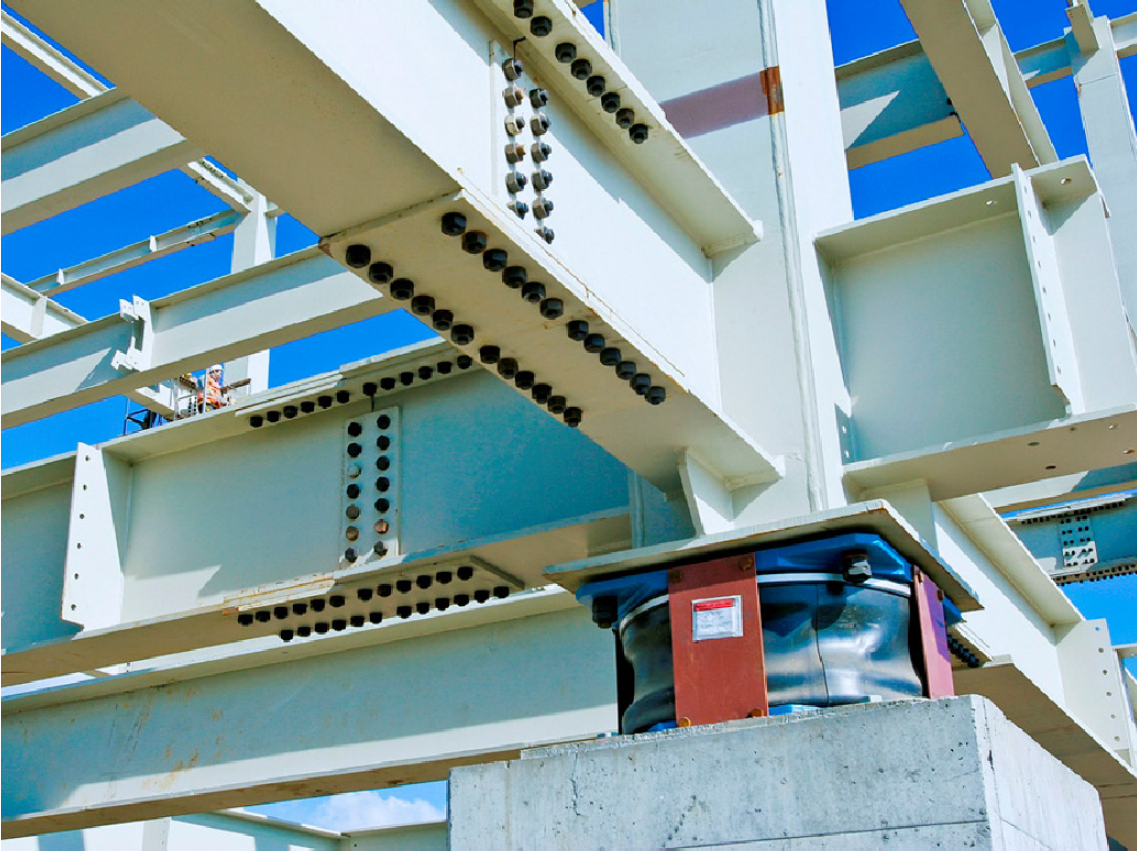
\includegraphics[height=5cm]{fig/a.PNG} \hspace{1cm}
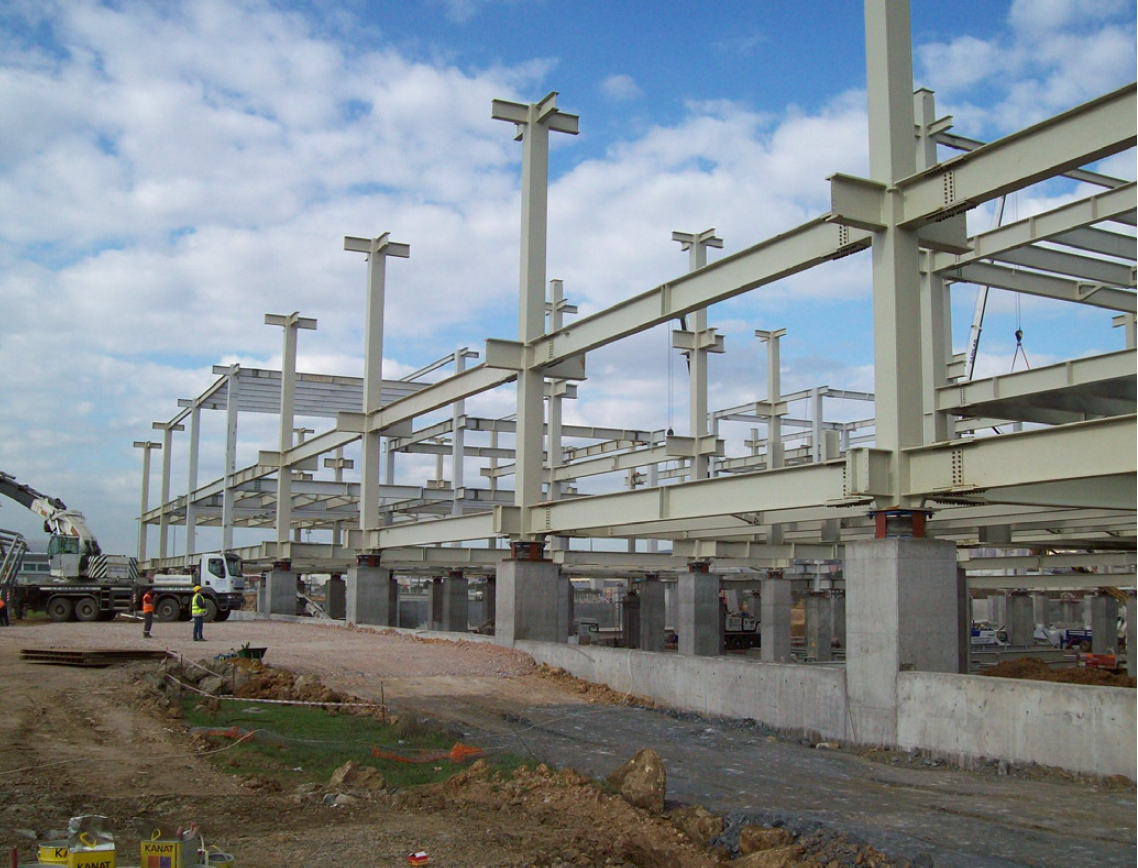
\includegraphics[height=5cm]{fig/b.PNG} \vspace{6pt}
 \caption{\label{fig:SabihaG=0000F6k=0000E7en} Sabiha Gökçen Uluslararası Havalimanına
ait sismik izolatör kolon kiriş birleşimi ve çelik üst yapı \cite{Zekioglu2009}.}
\end{figure}

\newpage{}

\section{Problemin Tanımı}

Sismik yalıtımlı yapıların tasarımı, doğrusal yöntemlerle ön boyutlandırma
aşaması ve doğrusal olmayan dinamik analizlerle tasarımın doğrulanması
olmak üzere iki aşamalıdır. Ön tasarım aşamasında eşdeğer doğrusal
analiz ve mod birleştirme yöntemleri kullanılmaktadır.

Sismik yalıtımlı yapılarda izolatörlerin hakim frekansları ile tabanı
ankastre kabul edilen üst yapı frekansları belirgin biçimde ayrıklaşır.
Göreli olarak düşük yatay rijitliğe sahip yalıtım birimleri, üst yapının
yapacağı deformasyonları azaltmaktadır. Bu nedenlerle elastik sınırlar
içerisinde davranması beklenen yapının, yapısal düzensizliklerinin
bulunmaması halinde gerekli idealleştirmeler yapılarak sistem basitleştirilebilir.
Ayrıca yapının sahip olduğu doğrusal olmayan dinamik özellikler, idealleştirilmiş
sisteme karşılık gelen parametrelerle ifade edilebilir. Eşdeğer doğrusal
analiz yönteminde tüm yapı, Şekil \ref{fig:equivalentmodel}'de belirtildiği
gibi tek serbestlik dereceli bir sistem olarak temsil edilmektedir.
\begin{figure}[h!]
\centering{}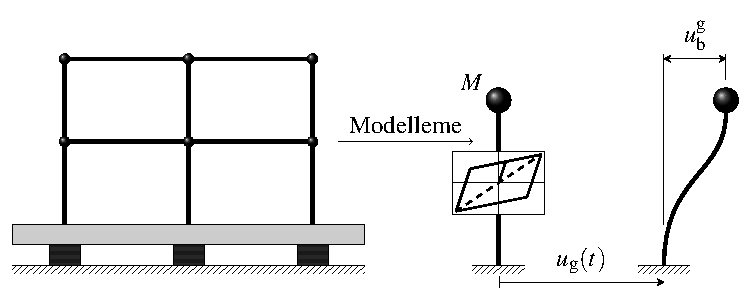
\includegraphics{TikZ/StructuralEquivalentModel} \caption{\label{fig:equivalentmodel} Eşdeğer Tek Serbestlik Dereceli Sistem.}
\end{figure}

Sismik yalıtımlı yapı sisteminin, tasarlanacağı yönetmelikte eşdeğer
doğrusal analiz için belirtilen uygulama sınırları dışında kalması
durumunda veya üst yapı taşıyıcı sisteminin sahip olduğu serbestlik
dereceleri de dikkate alınarak daha detaylı bir çözüm yapılmak istendiğinde
mod birleştirme yöntemi tercih edilmektedir. Üst yapının çok serbestlik
dereceli sistem olarak modellendiği bu yöntemde, izolatörlerin temsil
edildiği doğrusal kesme yaylarında eşdeğer rijitlik değerleri kullanılmaktadır.
Böylece kütlesi ve rijitliği belli olan sistemin doğrusal mod şekilleri
ve bu modlara karşılık gelen periyot ve frekans değerleri hesaplanır.
Tüm modlardan elde edilen iç kuvvet ve yer değiştirmeler birleştirilerek
sistemin deprem etkileri hesaplanır.

Doğrusal yöntemlerle tasarımı tamamlanan sismik yalıtımlı yapıların
kontrolü, geçmiş depremlerden elde edilen veya bölgenin depremsellik
özelliklerine uygun biçimde yapay olarak üretilen yer ivmeleri etkisinde,
yapıların doğrusal olmayan davranışlarının modellendiği, zaman tanım
alanında yapılan analizler ile sağlanır. İzolatör birimleri için kullanılan
kesme yaylarında doğrusal olmayan davranışların çeşitli malzeme modelleri
ile ifade edilebileceği gibi, eksenel yaylar, eğilme ve burulma yayları
da tanımlanabilmektedir. Ayrıca bu yayların birbirleri ile bağlı olarak
çalışması gerçeğe daha yakın analiz sonuçlarının elde edilmesini sağlamaktadır.
Bu analizde yapısal davranışlar, kütle ve rijitliklerin yanında yer
hareketlerinin içeriğine de bağlı olarak değişkenlik göstermektedir.
Bu nedenle yapının doğrusal olmayan dinamik analizinde, tasarımda
uyulan yönetmelik koşullarında belirtilen sayıda ve tasarım spektrumuna
göre ölçeklenmiş veya eşlenmiş yer ivmesi kullanılarak bulunan sonuçların
ortalaması değerlendirilmektedir.

Sismik yalıtımlı yapıların tasarım metotları 1970'lerden günümüze
kadar fiziksel deneyler veya analitik modellerden elde edilen bilgiler
ışığında pek çok kez irdelenmiştir. Yapılan araştırmalar içinde doğrusal
tasarım metotlarının geçerliliği, kullanım sınırları ve doğruluk mertebeleri
incelenen konular arasında bulunmaktadır. Sismik yalıtımlı yapıların
tasarımında kullanılan doğrusal yöntemler, konvansiyonel yapılardan
farklı olarak yalnızca ön tasarım aşamasında kullanılmaktadır. Öngörülen
en büyük depremden sonra dahi yapının kesintisiz olarak kullanılma
gerekliliği, yapısal tasarımda gerçeğe en yakın sonuçların elde edilmesini
sağlayacak analizlerin uygulanma zorunluluğunu da beraberinde getirmektedir.
Dolayısıyla ana hatları doğrusal analizler ile belirlenen sismik yalıtımlı
sistem tasarımlarının, bölgenin depremselliğine uygun olarak seçilecek
deprem kayıtları kullanılarak yapılacak doğrusal olmayan dinamik analizler
sayesinde kontrol edilerek son hale getirilmesi önemlidir. Fakat bu
ileri seviye analizler, karmaşık olabilmekte ve uzun zaman almaktadır.
Bu nedenle, son aşamaya kadar doğrusal yöntemler ile ilerletilen sismik
yalıtımlı yapı projelerinde bu analizlerin doğruluğu önem arz etmektedir.
İlerleyen başlıklarda doğrusal analiz yöntemleri irdelenmiştir.

\section{Amaç ve Kapsam}

\label{EquivalentLinearAnalysis} Eşdeğer doğrusal analiz yönteminde
kullanılan sistemde izolatörlerin üzerinde bulunan yalıtım düzlemi
ve üst yapı, tek bir kütle olarak değerlendirilmektedir. İzolatör
eşdeğer rijitliği, her bir izolatör biriminin tasarım deplasmanı için
elde edilecek sekant rijitlikleri toplamını belirtmektedir. Buna bağlı
olarak izolatör periyodu, tek serbestlik dereceli sistem için hesaplanmaktadır.
Sistemin sönümleyeceği enerji ise izolatörlerin doğrusal olmayan histeretik
davranışlarından elde edilecek eşdeğer viskoz sönüm oranı cinsinden
ifade edilir. Eşdeğer doğrusal analiz yöntemi, içerdiği kabul ve idealleştirmeler
sebebi ile kullanılan yönetmeliklerde belirtilen kriterlerin sağlanması
durumunda uygulanabilmektedir.

Ön tasarım aşamasında izolatörlerde meydana gelecek en büyük yatay
yer değiştirme değerinin tespit edilmesi izolatör boyutlarının belirlenmesinde
önemli bir kriterdir. En büyük yer değiştirme değeri, en büyük izolatör
kuvvetinin eşdeğer rijitliğe bölümü ile bulunmaktadır. Fakat eşdeğer
rijitlik değerinin belirlenebilmesi, izolatörün en büyük yer değiştirme
değerinin bilinmesi ile mümkün olmaktadır. Ön tasarımın ilk adımında
oluşan bu belirsizlik, detayları Bölüm \ref{CH2}'de sunulan iterasyonlar
ile ortadan kaldırılmaktadır.

Üst yapının ön tasarımı için gerekli taban kesme kuvveti, bu yöntemde
yalıtım düzleminde oluşan kesme kuvvetine göre hesaplanmaktadır. Tasarımda
takip edilen yönetmeliğe bağlı olarak taban kesme kuvvetinin belirlenmesi
ve bu kuvvetin üst yapı katlarına dağıtılma biçimi farklılık göstermektedir.
EN 1998-1:2004'e göre, katlara etkiyen yatay kuvvetler eşdeğer periyot
ve sönüme göre hesaplanacak spektral ivmenin, ilgili kat kütlesi ile
çarpımından elde edilmektedir\cite{Eurocode2004}. Burada kat kütlelerinin
eşit olduğu kabulü yapılırsa kesme kuvvetlerinin katlara eşit miktarda
dağıtıldığı görülmektedir. Ayrıca yalıtım birimi seviyesinde meydana
gelen kesme kuvvetinin yapı kütlesine oranı ile üst yapı taban kesme
kuvvetinin üst yapı toplam kütlesine oranı eşit olmaktadır.

ASCE/SEI-7-10 (2010) ve TBDY (2018) yönetmeliklerinde yer alan formüle
göre taban kesme kuvveti, yalıtım seviyesinde oluşan kesme kuvvetine
eşit alınarak üst yapı katlarına üçgen formunda dağıtılmaktadır \cite{ASCE2010,TBDY2018}.

ASCE/SEI-41-13 (2014) ve ASCE/SEI-7-16 (2016) yönetmeliklerinde ise
yalıtım düzleminde oluşacak kesme kuvveti, yapı taban kesme kuvvetine
eşit olarak alınmamaktadır \cite{ASCE41-13,ASCE2016}. York ve Ryan
tarafından yapılan çalışma, eşdeğer viskoz sönüm oranının artması
halinde, yapı taban kesme kuvvetinin yalıtım düzleminde oluşan kesme
kuvvetine oranının da artacağını göstermektedir \cite{doi:10.1080/13632460802003751}.
Buna bağlı olarak önerilen formül, istatistiksel parametreyi temsil
eden katsayıda bulunan değişiklik ile birlikte bu güncel yönetmeliklerde
yer almaktadır. Elde edilen artırılmış taban kesme kuvveti ise katlara
çalışmada önerilen formülün güncel haline göre paylaştırılmaktadır.

TBDY (2018) yönetmeliğine göre hesaplanacak taban kesme kuvvetinde
belirlenecek deprem yükü azaltma katsayısı $R$, hedeflenecek kesintisiz
kullanım ve sınırlı hasar performans düzeyleri için dayanım fazlalığı
katsayısı $D$ ile eşit verilmektedir \cite{TBDY2018}. Benzer olarak
ASCE/SEI-7-10 (2010) yönetmeliğinde belirtilen formülde yer alan $R_{1}$
katsayısı, üst yapı yatay taşıyıcı sistemine bağlı olarak belirlenecek
$R$ katsayısının $3/8$'i alınarak hesaplanmakta ve en fazla $2$
olarak belirlenebilmektedir \cite{ASCE2010}. Dolayısıyla $R_{1}$
katsayısı, hiçbir taşıyıcı sistem için dayanım fazlalığı katsayısı
$\Omega_{\text{0}}$'dan büyük olmamaktadır. Böylece yapının karşılaşması
beklenen en büyük deprem etkisi altında elastik sınırlar içinde kalması,
yalnızca eşdeğer doğrusal analiz yönteminin belirlediği kabuller çerçevesinde,
yalıtım düzlemi kesme kuvvetinin üst yapı taban kesme kuvvetine eşit
olması durumunda mümkün olmaktadır.



\chapter{YARI-RİJİT BİRLEŞİMLER}

\label{CH2} 

\section{Birleşimlerin Sınıflandırılması}

Bu bölümde, ortak yalıtım düzleminde bulunan sismik yalıtımlı tekli
ve çoklu yapılara ait hareket denklemleri, çalışmada kullanılacak
hali ile yeniden türetilmiş ve ardından hareket denklemlerinin çalışma
kapsamında kullanılan doğrusal olmayan çözüm yöntemine ait detaylar
verilmiştir. Bununla birlikte sismik yalıtımlı yapıların analizinde
kullanılan sönüm modellerine ait detaylar paylaşılmıştır. Ayrıca sismik
yalıtımlı yapıların eşdeğer doğrusal analizine ilişkin tasarım metodolojileri
ilgili yöntem ve yönetmelikler dahilinde açıklanmıştır.

\section{Birleşim Davranışının Modellenmesi}

\label{eom-singlestructure} Nagarajaiah ve diğerleri tarafından sunulan
sismik yalıtımlı tek yapılara ait hareket denklemlerinde, her bir
kat 3 serbestlik derecesi ile ifade edilmektedir \cite{doi:10.1061/(ASCE)0733-9445(1991)117:7(2035)}.
Bu çalışma kapsamında, tek doğrultuda yatay ötelenme serbestlik dereceleri
dikkate alınacaktır. Bu sebeple hareket denklemleri, çalışma kapsamında
kullanılacak sınırlar çerçevesinde detaylı olarak açıklanmıştır. Denklemler,
kütleleri kat hizalarında toplanmış olan ve yalnızca yatay kesme yaylarının
yapı rijitliğini temsil ettiği örnek sismik yalıtımlı sistem üzerinden
türetilmiştir. 
\begin{figure}[h!]
\centering{}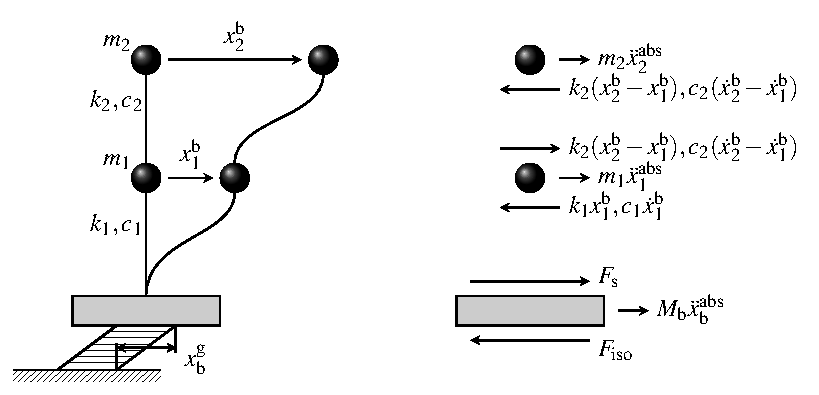
\includegraphics{TikZ/SingleStructureAndFBD} \caption{\label{fig:singlestructurefbd}Sismik yalıtımlı tek yapının şekil
değiştirmiş hali ve serbest cisim diyagramı.}
\end{figure}

Şekil \ref{fig:singlestructurefbd}'de yapının temsili şekil değiştirmiş
hali ile dinamik yükleme altında katlara ve yalıtım düzlemine etkiyen
kuvvetler sunulmuştur. Burada, $x^{\text{b}}$ katların yalıtım düzlemine
göre bağıl yer değiştirmelerini, $x_{\text{b}}^{\text{g}}$ yalıtım
düzleminin zemine göre bağıl yer değiştirmesini, $m$ kat kütlelerini,
$m_{\text{b}}$ yalıtım düzlemi kütlesini, $k$ kat rijitliklerini,
$c$ ilgili kata ait sönüm değerini, $F_{\text{s}}$ yapının taban
kesme kuvvetini, $F_{\text{iso}}$ izolatör seviyesinde oluşan kesme
kuvvetini ve noktalar ise zamana bağlı türevi belirtmektedir. Terimlerde
alt indis şeklinde bulunan numaralar, ilgili büyüklüğün hangi kata
ait olduğunu göstermektedir. Buna göre, yapının ilk katına ait hareket
denklemi \ref{eq-eom-1}'deki gibi ifade edilebilir. 
\begin{equation}
-k_{2}\left[x_{2}^{\text{b}}-x_{1}^{\text{b}}\right]+k_{1}x_{1}^{\text{b}}-c_{2}\left[\dot{x}_{2}^{\text{b}}-\dot{x}_{1}^{\text{b}}\right]+c_{1}\dot{x}_{1}^{\text{b}}=-m_{1}\ddot{x}_{1}^{\text{abs}}\label{eq-eom-1}
\end{equation}
Dinamik denge, D'Alembert prensibine göre yazılmıştır. Bu prensibe
göre, sisteme etkiyen kuvvetlerin yanı sıra, fiktif atalet kuvvetlerinin
ivme yönüne ters olarak eklenmesi halinde sistem her zaman anı için
denge durumunda bulunmaktadır. Dolayısıyla eşitliğin sağ tarafında
yer alan $\ddot{x}_{1}^{\text{abs}}$ terimi, aşağıdaki denklemde
belirtildiği gibi yalıtım düzleminde oluşan ve $\ddot{x}_{\text{b}}^{\text{abs}}$
ile ifade edilen ivmeler ile, dinamik dengenin sağlanabilmesi için
denkleme eklenen fiktif $\ddot{x}_{1}^{\text{b}}$ ivmesinin toplamını
ifade etmektedir. 
\begin{equation}
\ddot{x}_{1}^{\text{abs}}=\ddot{x}_{1}^{\text{b}}+\ddot{x}_{\text{b}}^{\text{abs}}\label{eq-acc-1}
\end{equation}
Benzer şekilde yapının ikinci katına ait hareket denklemi ve $\ddot{x}_{2}^{\text{abs}}$
teriminin açılımı aşağıda sunulmuştur. 
\begin{equation}
k_{2}\left[x_{2}^{\text{b}}-x_{1}^{\text{b}}\right]+c_{2}\left[\dot{x}_{2}^{\text{b}}-\dot{x}_{1}^{\text{b}}\right]=-m_{2}\ddot{x}_{2}^{\text{abs}}\label{eq-eom-2}
\end{equation}
\begin{equation}
\ddot{x}_{2}^{\text{abs}}=\ddot{x}_{2}^{\text{b}}+\ddot{x}_{\text{b}}^{\text{abs}}\label{eq-acc-2}
\end{equation}
Yukarıda verilen denklemler düzenlenerek matris formunda yazılırsa
aşağıda sunulan denklem elde edilir. 
\begin{equation}
\begin{split}\begin{bmatrix}m_{1} & 0\\
0 & m_{2}
\end{bmatrix}\begin{Bmatrix}\ddot{x}_{1}^{\text{b}}\\
\ddot{x}_{2}^{\text{b}}
\end{Bmatrix}+ & \begin{bmatrix}c_{1}+c_{2} & -c_{2}\\
-c_{2} & c_{2}
\end{bmatrix}\begin{Bmatrix}\dot{x}_{1}^{\text{b}}\\
\dot{x}_{2}^{\text{b}}
\end{Bmatrix}+\begin{bmatrix}k_{1}+k_{2} & -k_{2}\\
-k_{2} & k_{2}
\end{bmatrix}\begin{Bmatrix}{x}_{1}^{\text{b}}\\
{x}_{2}^{\text{b}}
\end{Bmatrix}=\\
 & -\begin{bmatrix}m_{1} & 0\\
0 & m_{2}
\end{bmatrix}\begin{Bmatrix}1\\
1
\end{Bmatrix}\ddot{x}_{\text{b}}^{\text{abs}}
\end{split}
\label{eq-eom-singlestructure}
\end{equation}
Aşağıdaki denklemde açıklandığı üzere $\ddot{x}_{\text{b}}^{\text{abs}}$
terimi, $\ddot{x}_{\text{b}}^{\text{g}}$ ile ifade edilen yalıtım
düzleminin zemine göre bağıl ivmesi ile $\ddot{x}_{\text{g}}^{\text{abs}}$
ifadesine karşılık gelen yer ivmesinin toplamını belirtmektedir. 
\begin{equation}
\ddot{x}_{\text{b}}^{\text{abs}}=\ddot{x}_{\text{b}}^{\text{g}}+\ddot{x}_{\text{g}}^{\text{abs}}\label{eq-abs-base-acc}
\end{equation}
Yalıtım düzlemine göre bağıl olarak ifade edilmiş olan yapının hareket
denklemi kapalı formda aşağıdaki gibi yazılabilir. 
\begin{equation}
\mathbf{M}_{\text{s}}\mathbf{\ddot{x}}_{\text{s}}^{\text{b}}+\mathbf{C}_{\text{s}}\mathbf{\dot{x}}_{\text{s}}^{\text{b}}+\mathbf{K}_{\text{s}}^{\text{b}}\mathbf{x}_{\text{s}}^{\text{b}}=-\mathbf{M}_{\text{s}}\mathbf{R}\ddot{x}_{\text{b}}^{\text{g}}-\mathbf{M}_{\text{s}}\mathbf{R}\ddot{x}_{\text{g}}^{\text{abs}}\label{eq-eom-singlestructure-closed}
\end{equation}
Burada, $\mathbf{M}_{\text{s}}$ kütle, $\mathbf{C}_{\text{s}}$ sönüm,
$\mathbf{K}_{\text{s}}$ rijitlik matrisini, $\mathbf{x}_{\text{s}}$
katların yalıtım düzlemine göre bağıl yer değiştirme vektörünü, $\mathbf{\ddot{x}}_{\text{b}}^{\text{g}}$
yalıtım düzleminin zemine göre bağıl ivmesini, $\mathbf{\ddot{x}}_{\text{g}}^{\text{abs}}$
yer ivmesini, $\mathbf{R}$ deprem etki vektörünü ve noktalar ise
zamana bağlı türevleri ifade etmektedir. Elde edilen üst yapı bağıl
hareket denkleminde deprem kuvvetlerini oluşturacak ivmeler, yalnızca
yalıtım düzleminin mutlak ivmesine eşittir. Dolayısıyla üst yapıya
etkiyen deprem kuvvetlerinde yer ivmelerinin doğrudan etkisi bulunmamaktadır.

Burada, $\mathbf{M}$, $\mathbf{C}$ ve $\mathbf{K}$ tüm yapıya ait
sırasıyla kütle, sönüm ve rijitlik matrislerini, $\mathbf{x}$ yapı
yer değiştirme vektörünü ve $\mathbf{S}_{\text{1}}$ ise etki vektörünü
ifade etmektedir. Denklemde belirtilen terimlerin açık hali aşağıda
verilmiştir. \vspace{0.2cm}

\begin{center}
$\mathbf{M}=\begin{bmatrix}\mathbf{M}_{\text{s}} & \mathbf{M}_{\text{s}}\mathbf{R}\\
\mathbf{R}^{\text{T}}\mathbf{M}_{\text{s}} & \mathbf{R}^{\text{T}}\mathbf{M}_{\text{s}}\mathbf{R}+M_{\text{b}}
\end{bmatrix}$ \hspace{0.2cm} $\mathbf{M}_{\text{s}}=\begin{bmatrix}m_{1} & 0\\
0 & m_{2}
\end{bmatrix}$ \vspace{0.25cm}
\par\end{center}

\begin{center}
$\mathbf{C}=\begin{bmatrix}\mathbf{C}_{\text{s}} & \mathbf{0}\\
\mathbf{0} & C_{\text{b}}
\end{bmatrix}$ \hspace{0.2cm} $\mathbf{C}_{\text{s}}=\begin{bmatrix}c_{1}+c_{2} & -c_{2}\\
-c_{2} & c_{2}
\end{bmatrix}$ \vspace{0.25cm}
\par\end{center}

\begin{center}
$\mathbf{K}=\begin{bmatrix}\mathbf{K}_{\text{s}} & \mathbf{0}\\
\mathbf{0} & K_{\text{b}}
\end{bmatrix}$ \hspace{0.2cm} $\mathbf{K}_{\text{s}}=\begin{bmatrix}k_{1}+k_{2} & -k_{2}\\
-k_{2} & k_{2}
\end{bmatrix}$ \vspace{0.25cm}
\par\end{center}

\begin{center}
$\mathbf{\ddot{x}}=\begin{Bmatrix}\mathbf{\ddot{x}}_{\text{s}}^{\text{b}}\\
\ddot{x}_{\text{b}}^{\text{g}}
\end{Bmatrix}$ \hspace{0.2cm} $\mathbf{\ddot{x}}_{\text{s}}^{\text{b}}=\begin{Bmatrix}\ddot{x}_{1}^{\text{b}}\\
\ddot{x}_{2}^{\text{b}}
\end{Bmatrix}$ \hspace{0.5cm} $\mathbf{\dot{x}}=\begin{Bmatrix}\mathbf{\dot{x}}_{\text{s}}^{\text{b}}\\
\dot{x}_{\text{b}}^{\text{g}}
\end{Bmatrix}$ \hspace{0.2cm} $\mathbf{\dot{x}}_{\text{s}}^{\text{b}}=\begin{Bmatrix}\dot{x}_{1}^{\text{b}}\\
\dot{x}_{2}^{\text{b}}
\end{Bmatrix}$ \hspace{0.5cm} $\mathbf{x}=\begin{Bmatrix}\mathbf{x}_{\text{s}}^{\text{b}}\\
{x}_{\text{b}}^{\text{g}}
\end{Bmatrix}$ \hspace{0.2cm} $\mathbf{x}_{\text{s}}^{\text{b}}=\begin{Bmatrix}{x}_{1}^{\text{b}}\\
{x}_{2}^{\text{b}}
\end{Bmatrix}$ \vspace{0.25cm}
\par\end{center}

\begin{center}
$\mathbf{S}_{\text{1}}=\begin{Bmatrix}\mathbf{0}\\
1
\end{Bmatrix}$ \hspace{0.2cm} $\mathbf{R}=\begin{Bmatrix}1\\
1
\end{Bmatrix}$ 
\par\end{center}

\newpage{}

\section{Birleşim Dönme Kapasitesi}

Sismik yalıtımlı çoklu yapılara ait hareket denklemleri Tsopelas ve
diğerleri tarafından açıklanmıştır \cite{TSOPELAS199447}. Yapılan
çalışmada, düzlem içi rijitlikleri sonsuz yapı katlarını temsil eden
toplu kütlelerin iki yatay ötelenme ve bir dönme olmak üzere toplam
üç adet serbestlik derecesi bulunmaktadır. Kütle merkezlerinde konumlanan
bu serbestlik dereceleri, yalıtım düzlemi kütle merkezinden geçen
düşey referans aksa göre eksantrik olarak tanımlanabilmektedir. Tez
çalışması kapsamında ortak yalıtım düzleminde bulunan çoklu yapıların
parametrik değişkenler altında yapı davranışları, yalnızca tek doğrultuda
yatay ötelenme serbestlik dereceleri dikkate alınarak incelenmiştir.
Bu sebeple hareket denklemleri, Şekil \ref{fig:multistructure}'de
sunulan örnek yapı üzerinden türetilecektir.

\section{Önceki Çalışmalar}

\begin{figure}[h]
\centering{}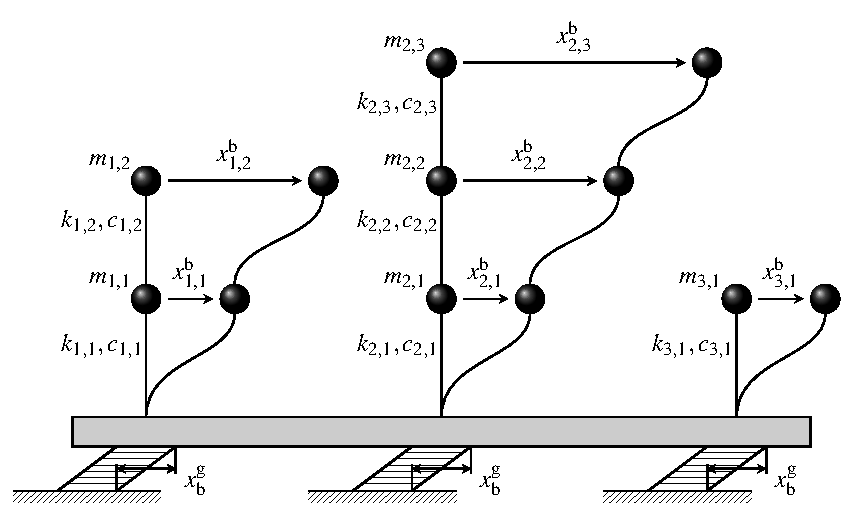
\includegraphics[width=1\linewidth]{TikZ/MultiStructure}
\caption{\label{fig:multistructure}Sismik yalıtımlı çoklu yapıların şekil
değiştirmiş hali.}
\end{figure}

Burada, $m$ kat kütlelerini, $c$ kat sönümünü, $k$ rijitlik değerini
ve $x$ ise yer değiştirmeleri belirtmektedir. Üst indiste büyüklüğün
göreli olarak yazıldığı konum belirtilmiştir. Yapı kat yer değiştirmelerinde
alt indislerde verilen ilk rakam yapı numarasını, ikinci rakam ise
büyüklüğün hangi kata ait olduğunu işaret etmektedir. Yalıtım düzlemi
yer değiştirmesi veya izolatör deplasmanları ise $x_{\text{b}}^{\text{g}}$
ile verilmiştir.



\chapter{DEPLASMAN ARTTIRMA KATSAYISI}

\label{CH3} 

Tez çalışması kapsamında sismik yalıtımlı yapıların doğrusal olmayan
hareket denklemlerinin yer ivmeleri etkisinde daha önce belirtilen
kapsam ve yöntemler dahilinde çözülebildiği MSBIS programı hazırlanmıştır.
Bu bölümde, oluşturulan algoritmanın doğrulaması yapılarak, yapısal
özellikleri açıklanmış ve ortak yalıtım düzleminde bulunan ikili yapıların,
parametrik incelenmesine dair prosedürler gösterilecektir. Daha sonra
hazırlanan çalışmaya ait sonuçlar paylaşılmıştır. Son olarak ikiden
fazla yapının ortak yalıtım düzleminde bulunması durumu için hazırlanan
örnek sistemler incelenecektir.

Numarasız denkleme örnek:

\section{Taşıyıcı Sistem Davranış Katsayısı}

Tez çalışması kapsamında sismik yalıtımlı yapıların doğrusal olmayan
hareket denklemlerinin yer ivmeleri etkisinde daha önce belirtilen
kapsam ve yöntemler dahilinde çözülebildiği MSBIS programı hazırlanmıştır.
Bu bölümde, oluşturulan algoritmanın doğrulaması yapılarak, yapısal
özellikleri açıklanmış ve ortak yalıtım düzleminde bulunan ikili yapıların,
parametrik incelenmesine dair prosedürler gösterilecektir. Daha sonra
hazırlanan çalışmaya ait sonuçlar paylaşılmıştır. Son olarak ikiden
fazla yapının ortak yalıtım düzleminde bulunması durumu için hazırlanan
örnek sistemler incelenecektir.

Numarasız denkleme örnek:
\[
\Delta=5x
\]


\section{Dayanım Fazlalığı Katsayısı}

\label{StructuralProperties} Tez çalışması kapsamında incelenen ortak
yalıtım düzleminde bulunan sismik yalıtımlı iki yapının değerlendirilmesi,
bu bölümde açıklanan yapı parametreleri kullanılarak gerçekleştirilmiştir.
Yapılar yalnızca yatay doğrusal kesme yaylarına sahip çok serbestlik
dereceli sistemlerden oluşmaktadır. Yapı elemanları, doğrusal elastik
olarak modellenmiştir. Dolayısıyla, üst yapı taşıyıcılarında deprem
yükleri altında oluşan kuvvet-yer değiştirme ilişkisinin doğrusal
elastik olduğu kabul edilmiştir. Şekil \ref{fig:structuralmodel}'de
belirtildiği gibi yalıtım düzlemi ve yapı kat döşemeleri düzlem içinde
rijit kabul edilerek tek bir kütle ile ifade edilmiştir. 
\begin{figure}[h!]
\centering{}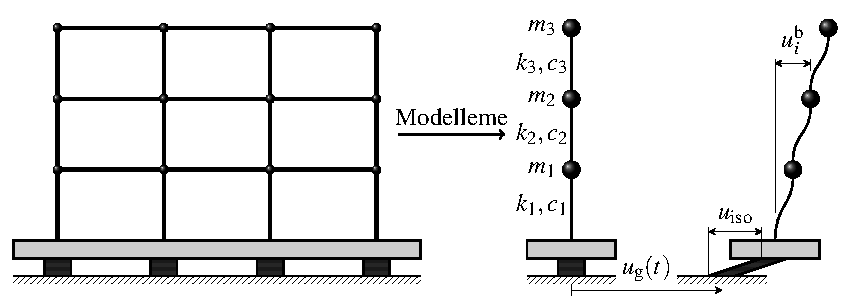
\includegraphics{TikZ/StructuralModel} \caption{\label{fig:structuralmodel}3 nolu yapıya ait analitik model ve yapının
şekil değiştirmiş hali.}
 
\end{figure}

Yapının kat rijitlikleri, tüm kolonların yatay rijitliklerinin denklem
\ref{lateralstiffness}'de verilen formüle göre belirlenerek toplanması
ile elde edilmiştir. Her bir kat için yatay rijitlik değeri, toplam
16 adet 60 $\times$ 60 cm boyutlarında betonarme kolonların yatay
rijitlikleri toplamına eşit olarak alınmıştır. Tüm yapı ve katlar
için kat yüksekliği h=4m olarak belirlenmiştir. Betonarme elastisite
modulü $E_{\text{c}}=32000\text{ MPa}$ olarak kabul edilmiştir. 
\begin{equation}
\sum\limits _{i=1}^{n}k_{i}=\dfrac{12E_{\text{c}}I}{h^{3}}\label{lateralstiffness}
\end{equation}
Burada, $k$ her bir kolona ait yatay rijitliği, $E_{\text{c}}$ betonarme
elastisite modulünü, $I$ atalet momentini, h kat yüksekliğini ve
n bir katta bulunan kolon adedini ifade etmektedir. Sismik yalıtım
sistemi ise tüm izolatörlerin yapısal özelliklerinin toplamı ile ifade
edilen doğrusal olmayan yatay kesme yayı ile tanımlanmıştır. Ayrıca
sismik yalıtımlı yapının sahip olduğu sönüm, izolatörlerin doğrusal
olmayan kesme yaylarında sönümlediği enerji ve üst yapının sahip olduğu
Rayleigh sönümü olmak üzere ayrıklaştırılmıştır. Yapısal sönüm modellerine
ait detaylar Bölüm detaylı olarak açıklanmıştır.

\section{Süneklik Azaltma Katsayısı}

sadsadasdasdaşkms alsdöaşsd 

\begin{table}[h]
\centering{}\caption{\label{structures2}Çalışma kapsamında incelenen sistemlerin tabanı
ankastre olması durumu için hesaplanan yapısal özellikleri.}
\begin{tabular}{ccccc}
\hline 
Yapı \#  & Kat Adedi  & $T_{1}$  & $\omega_{1}$  & $\omega_{\text{n}}$ \tabularnewline
\hline 
1  & 1  & 0.1573  & 39.94  & - \tabularnewline
2  & 2  & 0.2546  & 24.68  & 64.62 \tabularnewline
3  & 3  & 0.3535  & 17.77  & 71.97 \tabularnewline
4  & 4  & 0.4530  & 13.87  & 75.06 \tabularnewline
5  & 5  & 0.5527  & 11.37  & 76.64 \tabularnewline
6  & 6  & 0.6526  & 9.63  & 77.56 \tabularnewline
7  & 7  & 0.7525  & 8.35  & 78.13 \tabularnewline
8  & 8  & 0.8525  & 7.37  & 78.52 \tabularnewline
9  & 9  & 0.9525  & 6.60  & 78.79 \tabularnewline
10  & 10  & 1.0526  & 5.97  & 78.98 \tabularnewline
\hline 
\end{tabular}
\end{table}

Tez çalışması kapsamında ortak yalıtım düzleminde bulunan yapıların,
dinamik özelliklerinin taban kesme kuvvetlerine olan etkisini incelemek
üzere on adet yapı seçilmiştir. Kat sayıları birden ona kadar değişen
yapıların kat rijitlikleri $\text{k}_{i}=0.0108\text{ m}^{4}$, kat
kütleleri $m_{i}=650\text{ ton}$ ve üst yapıya ait sönüm oranları
$\xi=0.05$ olmak üzere tümünde aynıdır. Kat adedine bağlı olarak
değişen yapı doğal periyotları ile birinci ve sonuncu açısal frekans
değerleri Çizelge \ref{structures2}'de sunulmuştur. Ayrıca, yalıtım
düzlemi kütlesi her bir yapı için $m_{\text{b}}=981\text{ ton}$ olarak
alınmıştır. Yalıtım birimlerine ait dinamik özellikler parametrik
olarak belirlenmiş olup Bölüm'de detaylı olarak açıklanmıştır.

\section{Deplasman Arttırma Katsayısı}

adsadad

\section{Eşit Yerdeğiştirme ve Eşit Enerji Prensipleri}

sdasdalsdkalms



\chapter{PARAMETRİK ÇALIŞMA}

\section{Parametrik Çalışmada Kullanılacak Yapılar}

\label{CH4} 

Bu çalışmada ortak yalıtım düzleminde bulunan sismik yalıtımlı iki
yapı için parametrik bir çalışma yapılmıştır. Analizler bağımsız veya
ortak yalıtım düzleminde bulunan sismik yalıtımlı yapıların doğrusal
olmayan dinamik analizlerinin parametrik olarak yapılabildiği MSBIS
programı yardımıyla gerçekleştirilmiştir. Üst yapı yapısal özelliklerinin
parametrik olarak değiştiği analizlerin tamamı, yalıtım birimlerinin
farklı eşdeğer periyot ve sönüm değerleri için tekrarlanmıştır. Burada
ortak yalıtım düzleminde bulunan sismik yalıtımlı birinci yapının
yapısal özellikleri değişen ikinci yapı ve izolatör parametreleri
değişimi ile meydana gelen etkileşimlerini incelemek amaçlanmıştır.
Buna göre birinci yapıda oluşan kat kesme kuvvetlerinde, göreli kat
ötelemelerinde ve kat ivmelerinde oluşan değişim irdelenmiştir. Taban
kesme kuvvetinin üst yapıya dağılımı ise yalıtım birimlerinin değişen
dinamik özelliklerine göre belirlenmiştir. Ayrıca ortak yalıtım düzlemindeki
iki yapı için gerekli deprem derz mesafeleri doğrusal yöntemler ile
bulunan sonuçlarla kıyaslanmıştır.

Çalışmada elde edilen sonuçlara göre yalıtım birimlerinin artan eşdeğer
sönüm oranına karşılık gelen büyük doğrusalsızlık sebebi ile ortak
yalıtım düzleminde bulunan yapıların yüksek mod etkilerinin göreli
yer değiştirme ve iç kuvvetlerinde önemli artışlara sebep olduğu görülmüştür.
Bu artışların iki yapının açısal frekanslarının ayrıklaşması ile arttığı
tespit edilmiştir. Dolayısıyla iki yapının aynı açısal frekansa sahip
olması durumunda elde edilen iç kuvvet ve yer değiştirmeler, yalıtım
birimlerinin aynı eşdeğer periyot ve sönüm değerleri için eşit bulunmaktadır.
Bununla birlikte yalıtım birimlerinin artan eşdeğer sönüm değerleri
için sismik yalıtımlı yapı taban kesme kuvvetlerinin üst katlara dağılımında
meydana gelen dikdörtgen form yerini üst katlarda daha büyük kuvvetlerin
oluştuğu ters üçgen formuna bıraktığı görülmüştür.

\section{Yükler ve Yük Kombinasyonları}

Tez çalışması kapsamında elde edilen sonuçlar aşağıda listelenmiştir. 
\begin{enumerate}
\item Yalıtım birimlerinin sahip olduğu histeretik sönüm nedeniyle meydana
gelen yüksek mod etkisi doğrusal analizler ile bulunan sonuçların
değişmesine neden olmaktadır.
\item Ortak yalıtım düzleminde bulunan ve farklı açısal frekanslara sahip
yapıların şekil değiştirme ve iç kuvvetleri, bağımsız yalıtım düzleminde
bulunan aynı yapılara kıyasla artış göstermektedir.
\item Yapı taban kesme kuvvetlerinin üst katlara dağılımının eşdeğer sönüm
oranının artışı ile dikdörtgen formdan ters üçgen formuna doğru değiştiği
görülmüştür. Ayrıca iki yapının açısal frekanslarına bağlı olarak
bu değişimin artış veya azalışta olduğu tespit edilmiştir.
\item Deprem derz mesafelerinde doğrusal yöntemler ile bulunan değerlerin
yeterli olduğu tespit edilmiştir.
\item Ortak yalıtım düzleminde bulunan 1. yapı taban kesme kuvveti katsayısının
toplam taban kesme kuvveti katsayısına göre bağıl hatasının en büyük
değeri, 1 ve 10 katlı iki yapının ortak yalıtım düzleminde bulunması
durumunda ve $T_{\text{eff}}=$ 2.5sn ve $\xi_{\text{eff}}$=0.3 değerleri
için 2.20 olarak hesaplanmıştır.
\item Ortak yalıtım düzleminde bulunan yapıların taban kesme kuvveti katsayılarının
toplam taban kesme kuvveti katsayısına göre bağıl hatasının en büyük
değeri, 2 ve 10 katlı iki yapının ortak yalıtım düzleminde bulunması
durumunda ve $T_{\text{eff}}=$ 2.5sn ve $\xi_{\text{eff}}$=0.3 değerleri
için 1.20 olarak hesaplanmıştır.
\item Yalıtım birimi kesme kuvveti katsayısının ortak yalıtım düzleminde
bulunan yapıların toplam taban kesme kuvveti katsayısına göre bağıl
hatasının en büyük değeri, 1 ve 5 katlı iki yapının ortak yalıtım
düzleminde bulunması durumunda ve $T_{\text{eff}}=$ 2.5sn ve $\xi_{\text{eff}}$=0.3
değerleri için -0.218 olarak hesaplanmıştır.
\item 1 ve 10 katlı iki yapının ortak yalıtım düzleminde bulunması durumunda
$T_{\text{eff}}=$ 4sn ve $\xi_{\text{eff}}$=0.3 değerleri için,
1 katlı yapının kesme kuvveti kat ivmesi ve göreli kat ötelemesinin,
bağımsız yalıtım düzleminde bulunması durumuna göre 3.27 katına çıktığı
belirlenmiştir.
\item 1 ve 10 katlı iki yapının ortak yalıtım düzleminde bulunması durumunda
10 katlı yapının kat kesme kuvvetleri, bağımsız yalıtım düzleminde
bulunması durumuna göre alt katlarda en büyük azalma $T_{\text{eff}}=$
1.5sn ve $\xi_{\text{eff}}$=0.3 değerleri için \%21.6 ve üst katta
ise en büyük azalma $T_{\text{eff}}=$ 4sn ve $\xi_{\text{eff}}$=0.2
değerleri için \%18.9 olarak tespit edilmiştir.
\item 10 katlı yapının ortak yalıtım düzleminde bulunması durumunda kat
kesme kuvvetleri, bağımsız yalıtım düzleminde bulunması durumuna göre
alt katlarda en fazla \%53.1 artış $T_{\text{eff}}=$ 1.5sn ve $\xi_{\text{eff}}$=0.3
değerleri için 6 katlı yapı ile birlikte bulunması durumu için gerçekleşmiştir.
Ayrıca üst katta en büyük azalma $T_{\text{eff}}=$ 4sn ve $\xi_{\text{eff}}$=0.2
değerleri için 2 katlı yapı ile birlikte bulunmaları durumu için \%26.1
olarak saptanmıştır.
\item 10 katlı yapının ortak yalıtım düzleminde bulunması durumunda göreli
kat ötelemeleri, bağımsız yalıtım düzleminde bulunması durumuna göre
alt katlarda en fazla \%53.9 artış $T_{\text{eff}}=$ 1.5sn ve $\xi_{\text{eff}}$=0.3
değerleri için 6 katlı yapı ile birlikte bulunması durumu için gerçekleşmiştir.
Ayrıca üst katta en büyük azalma $T_{\text{eff}}=$ 4sn ve $\xi_{\text{eff}}$=0.2
değerleri için 2 katlı yapı ile birlikte bulunmaları durumu için \%26.4
olarak saptanmıştır. 
\end{enumerate}

\section{Moment Dayanımlı Çelik Çerçeveli Sistemlerin Tasarımı}

Tez çalışması kapsamında elde edilen sonuçlar aşağıda listelenmiştir.
Tez çalışması kapsamında elde edilen sonuçlar aşağıda listelenmiştir.
Tez çalışması kapsamında elde edilen sonuçlar aşağıda listelenmiştir.
Tez çalışması kapsamında elde edilen sonuçlar aşağıda listelenmiştir.
Tez çalışması kapsamında elde edilen sonuçlar aşağıda listelenmiştir.
Tez çalışması kapsamında elde edilen sonuçlar aşağıda listelenmiştir.
Tez çalışması kapsamında elde edilen sonuçlar aşağıda listelenmiştir.
Tez çalışması kapsamında elde edilen sonuçlar aşağıda listelenmiştir.
Tez çalışması kapsamında elde edilen sonuçlar aşağıda listelenmiştir.
Tez çalışması kapsamında elde edilen sonuçlar aşağıda listelenmiştir.
Tez çalışması kapsamında elde edilen sonuçlar aşağıda listelenmiştir.
Tez çalışması kapsamında elde edilen sonuçlar aşağıda listelenmiştir.
Tez çalışması kapsamında elde edilen sonuçlar aşağıda listelenmiştir.
Tez çalışması kapsamında elde edilen sonuçlar aşağıda listelenmiştir.
Tez çalışması kapsamında elde edilen sonuçlar aşağıda listelenmiştir.
Tez çalışması kapsamında elde edilen sonuçlar aşağıda listelenmiştir.
Tez çalışması kapsamında elde edilen sonuçlar aşağıda listelenmiştir.
Tez çalışması kapsamında elde edilen sonuçlar aşağıda listelenmiştir.
Tez çalışması kapsamında elde edilen sonuçlar aşağıda listelenmiştir.
Tez çalışması kapsamında elde edilen sonuçlar aşağıda listelenmiştir.
Tez çalışması kapsamında elde edilen sonuçlar aşağıda listelenmiştir.
Tez çalışması kapsamında elde edilen sonuçlar aşağıda listelenmiştir.
Tez çalışması kapsamında elde edilen sonuçlar aşağıda listelenmiştir.
Tez çalışması kapsamında elde edilen sonuçlar aşağıda listelenmiştir.
Tez çalışması kapsamında elde edilen sonuçlar aşağıda listelenmiştir.
Tez çalışması kapsamında elde edilen sonuçlar aşağıda listelenmiştir.
Tez çalışması kapsamında elde edilen sonuçlar aşağıda listelenmiştir.
Tez çalışması kapsamında elde edilen sonuçlar aşağıda listelenmiştir.
Tez çalışması kapsamında elde edilen sonuçlar aşağıda listelenmiştir.
Tez çalışması kapsamında elde edilen sonuçlar aşağıda listelenmiştir.
Tez çalışması kapsamında elde edilen sonuçlar aşağıda listelenmiştir.
Tez çalışması kapsamında elde edilen sonuçlar aşağıda listelenmiştir.
Tez çalışması kapsamında elde edilen sonuçlar aşağıda listelenmiştir.
Tez çalışması kapsamında elde edilen sonuçlar aşağıda listelenmiştir.
Tez çalışması kapsamında elde edilen sonuçlar aşağıda listelenmiştir.
Tez çalışması kapsamında elde edilen sonuçlar aşağıda listelenmiştir.
Tez çalışması kapsamında elde edilen sonuçlar aşağıda listelenmiştir.
Tez çalışması kapsamında elde edilen sonuçlar aşağıda listelenmiştir.
Tez çalışması kapsamında elde edilen sonuçlar aşağıda listelenmiştir.
Tez çalışması kapsamında elde edilen sonuçlar aşağıda listelenmiştir.
Tez çalışması kapsamında elde edilen sonuçlar aşağıda listelenmiştir.
Tez çalışması kapsamında elde edilen sonuçlar aşağıda listelenmiştir.
Tez çalışması kapsamında elde edilen sonuçlar aşağıda listelenmiştir.
Tez çalışması kapsamında elde edilen sonuçlar aşağıda listelenmiştir.
Tez çalışması kapsamında elde edilen sonuçlar aşağıda listelenmiştir.
Tez çalışması kapsamında elde edilen sonuçlar aşağıda listelenmiştir.
Tez çalışması kapsamında elde edilen sonuçlar aşağıda listelenmiştir.
Tez çalışması kapsamında elde edilen sonuçlar aşağıda listelenmiştir.
Tez çalışması kapsamında elde edilen sonuçlar aşağıda listelenmiştir.
Tez çalışması kapsamında elde edilen sonuçlar aşağıda listelenmiştir.
Tez çalışması kapsamında elde edilen sonuçlar aşağıda listelenmiştir.
Tez çalışması kapsamında elde edilen sonuçlar aşağıda listelenmiştir.
Tez çalışması kapsamında elde edilen sonuçlar aşağıda listelenmiştir.
Tez çalışması kapsamında elde edilen sonuçlar aşağıda listelenmiştir.
Tez çalışması kapsamında elde edilen sonuçlar aşağıda listelenmiştir.
Tez çalışması kapsamında elde edilen sonuçlar aşağıda listelenmiştir.
Tez çalışması kapsamında elde edilen sonuçlar aşağıda listelenmiştir.
Tez çalışması kapsamında elde edilen sonuçlar aşağıda listelenmiştir.
Tez çalışması kapsamında elde edilen sonuçlar aşağıda listelenmiştir.
Tez çalışması kapsamında elde edilen sonuçlar aşağıda listelenmiştir.
Tez çalışması kapsamında elde edilen sonuçlar aşağıda listelenmiştir.
Tez çalışması kapsamında elde edilen sonuçlar aşağıda listelenmiştir.
Tez çalışması kapsamında elde edilen sonuçlar aşağıda listelenmiştir.
Tez çalışması kapsamında elde edilen sonuçlar aşağıda listelenmiştir.
Tez çalışması kapsamında elde edilen sonuçlar aşağıda listelenmiştir.
Tez çalışması kapsamında elde edilen sonuçlar aşağıda listelenmiştir.
Tez çalışması kapsamında elde edilen sonuçlar aşağıda listelenmiştir.
Tez çalışması kapsamında elde edilen sonuçlar aşağıda listelenmiştir.
Tez çalışması kapsamında elde edilen sonuçlar aşağıda listelenmiştir.
Tez çalışması kapsamında elde edilen sonuçlar aşağıda listelenmiştir.
Tez çalışması kapsamında elde edilen sonuçlar aşağıda listelenmiştir.
Tez çalışması kapsamında elde edilen sonuçlar aşağıda listelenmiştir.
Tez çalışması kapsamında elde edilen sonuçlar aşağıda listelenmiştir.
Tez çalışması kapsamında elde edilen sonuçlar aşağıda listelenmiştir.
Tez çalışması kapsamında elde edilen sonuçlar aşağıda listelenmiştir.
Tez çalışması kapsamında elde edilen sonuçlar aşağıda listelenmiştir.
Tez çalışması kapsamında elde edilen sonuçlar aşağıda listelenmiştir.
Tez çalışması kapsamında elde edilen sonuçlar aşağıda listelenmiştir.
Tez çalışması kapsamında elde edilen sonuçlar aşağıda listelenmiştir.
Tez çalışması kapsamında elde edilen sonuçlar aşağıda listelenmiştir.
Tez çalışması kapsamında elde edilen sonuçlar aşağıda listelenmiştir.
Tez çalışması kapsamında elde edilen sonuçlar aşağıda listelenmiştir.
Tez çalışması kapsamında elde edilen sonuçlar aşağıda listelenmiştir.
Tez çalışması kapsamında elde edilen sonuçlar aşağıda listelenmiştir.
Tez çalışması kapsamında elde edilen sonuçlar aşağıda listelenmiştir.
Tez çalışması kapsamında elde edilen sonuçlar aşağıda listelenmiştir.
Tez çalışması kapsamında elde edilen sonuçlar aşağıda listelenmiştir.
Tez çalışması kapsamında elde edilen sonuçlar aşağıda listelenmiştir.
Tez çalışması kapsamında elde edilen sonuçlar aşağıda listelenmiştir.
Tez çalışması kapsamında elde edilen sonuçlar aşağıda listelenmiştir.
Tez çalışması kapsamında elde edilen sonuçlar aşağıda listelenmiştir.
Tez çalışması kapsamında elde edilen sonuçlar aşağıda listelenmiştir.
Tez çalışması kapsamında elde edilen sonuçlar aşağıda listelenmiştir.
Tez çalışması kapsamında elde edilen sonuçlar aşağıda listelenmiştir.
Tez çalışması kapsamında elde edilen sonuçlar aşağıda listelenmiştir.
Tez çalışması kapsamında elde edilen sonuçlar aşağıda listelenmiştir.
Tez çalışması kapsamında elde edilen sonuçlar aşağıda listelenmiştir.
Tez çalışması kapsamında elde edilen sonuçlar aşağıda listelenmiştir.
Tez çalışması kapsamında elde edilen sonuçlar aşağıda listelenmiştir.
Tez çalışması kapsamında elde edilen sonuçlar aşağıda listelenmiştir.
Tez çalışması kapsamında elde edilen sonuçlar aşağıda listelenmiştir.
Tez çalışması kapsamında elde edilen sonuçlar aşağıda listelenmiştir.
Tez çalışması kapsamında elde edilen sonuçlar aşağıda listelenmiştir.
Tez çalışması kapsamında elde edilen sonuçlar aşağıda listelenmiştir.
Tez çalışması kapsamında elde edilen sonuçlar aşağıda listelenmiştir.
Tez çalışması kapsamında elde edilen sonuçlar aşağıda listelenmiştir.
Tez çalışması kapsamında elde edilen sonuçlar aşağıda listelenmiştir.
Tez çalışması kapsamında elde edilen sonuçlar aşağıda listelenmiştir.
Tez çalışması kapsamında elde edilen sonuçlar aşağıda listelenmiştir.
Tez çalışması kapsamında elde edilen sonuçlar aşağıda listelenmiştir.
Tez çalışması kapsamında elde edilen sonuçlar aşağıda listelenmiştir.
Tez çalışması kapsamında elde edilen sonuçlar aşağıda listelenmiştir.
Tez çalışması kapsamında elde edilen sonuçlar aşağıda listelenmiştir.
Tez çalışması kapsamında elde edilen sonuçlar aşağıda listelenmiştir.
Tez çalışması kapsamında elde edilen sonuçlar aşağıda listelenmiştir.
Tez çalışması kapsamında elde edilen sonuçlar aşağıda listelenmiştir.
Tez çalışması kapsamında elde edilen sonuçlar aşağıda listelenmiştir.
Tez çalışması kapsamında elde edilen sonuçlar aşağıda listelenmiştir.
Tez çalışması kapsamında elde edilen sonuçlar aşağıda listelenmiştir.
Tez çalışması kapsamında elde edilen sonuçlar aşağıda listelenmiştir.
Tez çalışması kapsamında elde edilen sonuçlar aşağıda listelenmiştir.
Tez çalışması kapsamında elde edilen sonuçlar aşağıda listelenmiştir.
Tez çalışması kapsamında elde edilen sonuçlar aşağıda listelenmiştir.
Tez çalışması kapsamında elde edilen sonuçlar aşağıda listelenmiştir.
Tez çalışması kapsamında elde edilen sonuçlar aşağıda listelenmiştir.
Tez çalışması kapsamında elde edilen sonuçlar aşağıda listelenmiştir.
Tez çalışması kapsamında elde edilen sonuçlar aşağıda listelenmiştir.
Tez çalışması kapsamında elde edilen sonuçlar aşağıda listelenmiştir.
Tez çalışması kapsamında elde edilen sonuçlar aşağıda listelenmiştir.
Tez çalışması kapsamında elde edilen sonuçlar aşağıda listelenmiştir.
Tez çalışması kapsamında elde edilen sonuçlar aşağıda listelenmiştir.
Tez çalışması kapsamında elde edilen sonuçlar aşağıda listelenmiştir.
Tez çalışması kapsamında elde edilen sonuçlar aşağıda listelenmiştir.
Tez çalışması kapsamında elde edilen sonuçlar aşağıda listelenmiştir.
Tez çalışması kapsamında elde edilen sonuçlar aşağıda listelenmiştir.
Tez çalışması kapsamında elde edilen sonuçlar aşağıda listelenmiştir.
Tez çalışması kapsamında elde edilen sonuçlar aşağıda listelenmiştir.
Tez çalışması kapsamında elde edilen sonuçlar aşağıda listelenmiştir.
Tez çalışması kapsamında elde edilen sonuçlar aşağıda listelenmiştir.
Tez çalışması kapsamında elde edilen sonuçlar aşağıda listelenmiştir.
Tez çalışması kapsamında elde edilen sonuçlar aşağıda listelenmiştir.
Tez çalışması kapsamında elde edilen sonuçlar aşağıda listelenmiştir.
Tez çalışması kapsamında elde edilen sonuçlar aşağıda listelenmiştir.
Tez çalışması kapsamında elde edilen sonuçlar aşağıda listelenmiştir.
Tez çalışması kapsamında elde edilen sonuçlar aşağıda listelenmiştir.
Tez çalışması kapsamında elde edilen sonuçlar aşağıda listelenmiştir.
Tez çalışması kapsamında elde edilen sonuçlar aşağıda listelenmiştir.
Tez çalışması kapsamında elde edilen sonuçlar aşağıda listelenmiştir.
Tez çalışması kapsamında elde edilen sonuçlar aşağıda listelenmiştir.
Tez çalışması kapsamında elde edilen sonuçlar aşağıda listelenmiştir.
Tez çalışması kapsamında elde edilen sonuçlar aşağıda listelenmiştir.
Tez çalışması kapsamında elde edilen sonuçlar aşağıda listelenmiştir.
Tez çalışması kapsamında elde edilen sonuçlar aşağıda listelenmiştir.
Tez çalışması kapsamında elde edilen sonuçlar aşağıda listelenmiştir.
Tez çalışması kapsamında elde edilen sonuçlar aşağıda listelenmiştir.
Tez çalışması kapsamında elde edilen sonuçlar aşağıda listelenmiştir.
Tez çalışması kapsamında elde edilen sonuçlar aşağıda listelenmiştir.
Tez çalışması kapsamında elde edilen sonuçlar aşağıda listelenmiştir.
Tez çalışması kapsamında elde edilen sonuçlar aşağıda listelenmiştir.
Tez çalışması kapsamında elde edilen sonuçlar aşağıda listelenmiştir.
Tez çalışması kapsamında elde edilen sonuçlar aşağıda listelenmiştir.
Tez çalışması kapsamında elde edilen sonuçlar aşağıda listelenmiştir.
Tez çalışması kapsamında elde edilen sonuçlar aşağıda listelenmiştir.
Tez çalışması kapsamında elde edilen sonuçlar aşağıda listelenmiştir.
Tez çalışması kapsamında elde edilen sonuçlar aşağıda listelenmiştir.
Tez çalışması kapsamında elde edilen sonuçlar aşağıda listelenmiştir.
Tez çalışması kapsamında elde edilen sonuçlar aşağıda listelenmiştir.
Tez çalışması kapsamında elde edilen sonuçlar aşağıda listelenmiştir.
Tez çalışması kapsamında elde edilen sonuçlar aşağıda listelenmiştir.
Tez çalışması kapsamında elde edilen sonuçlar aşağıda listelenmiştir.
Tez çalışması kapsamında elde edilen sonuçlar aşağıda listelenmiştir.
Tez çalışması kapsamında elde edilen sonuçlar aşağıda listelenmiştir.
Tez çalışması kapsamında elde edilen sonuçlar aşağıda listelenmiştir.
Tez çalışması kapsamında elde edilen sonuçlar aşağıda listelenmiştir.
Tez çalışması kapsamında elde edilen sonuçlar aşağıda listelenmiştir.
Tez çalışması kapsamında elde edilen sonuçlar aşağıda listelenmiştir.
Tez çalışması kapsamında elde edilen sonuçlar aşağıda listelenmiştir.
Tez çalışması kapsamında elde edilen sonuçlar aşağıda listelenmiştir.
Tez çalışması kapsamında elde edilen sonuçlar aşağıda listelenmiştir.
Tez çalışması kapsamında elde edilen sonuçlar aşağıda listelenmiştir.
Tez çalışması kapsamında elde edilen sonuçlar aşağıda listelenmiştir.
Tez çalışması kapsamında elde edilen sonuçlar aşağıda listelenmiştir.
Tez çalışması kapsamında elde edilen sonuçlar aşağıda listelenmiştir.
Tez çalışması kapsamında elde edilen sonuçlar aşağıda listelenmiştir.
Tez çalışması kapsamında elde edilen sonuçlar aşağıda listelenmiştir.
Tez çalışması kapsamında elde edilen sonuçlar aşağıda listelenmiştir.
Tez çalışması kapsamında elde edilen sonuçlar aşağıda listelenmiştir.
Tez çalışması kapsamında elde edilen sonuçlar aşağıda listelenmiştir.
Tez çalışması kapsamında elde edilen sonuçlar aşağıda listelenmiştir.
Tez çalışması kapsamında elde edilen sonuçlar aşağıda listelenmiştir.
Tez çalışması kapsamında elde edilen sonuçlar aşağıda listelenmiştir.
Tez çalışması kapsamında elde edilen sonuçlar aşağıda listelenmiştir.
Tez çalışması kapsamında elde edilen sonuçlar aşağıda listelenmiştir.
Tez çalışması kapsamında elde edilen sonuçlar aşağıda listelenmiştir.
Tez çalışması kapsamında elde edilen sonuçlar aşağıda listelenmiştir.
Tez çalışması kapsamında elde edilen sonuçlar aşağıda listelenmiştir.
Tez çalışması kapsamında elde edilen sonuçlar aşağıda listelenmiştir.
Tez çalışması kapsamında elde edilen sonuçlar aşağıda listelenmiştir.
Tez çalışması kapsamında elde edilen sonuçlar aşağıda listelenmiştir.
Tez çalışması kapsamında elde edilen sonuçlar aşağıda listelenmiştir.
Tez çalışması kapsamında elde edilen sonuçlar aşağıda listelenmiştir.
Tez çalışması kapsamında elde edilen sonuçlar aşağıda listelenmiştir.
Tez çalışması kapsamında elde edilen sonuçlar aşağıda listelenmiştir.
Tez çalışması kapsamında elde edilen sonuçlar aşağıda listelenmiştir.
Tez çalışması kapsamında elde edilen sonuçlar aşağıda listelenmiştir.
Tez çalışması kapsamında elde edilen sonuçlar aşağıda listelenmiştir.
Tez çalışması kapsamında elde edilen sonuçlar aşağıda listelenmiştir.
Tez çalışması kapsamında elde edilen sonuçlar aşağıda listelenmiştir.
Tez çalışması kapsamında elde edilen sonuçlar aşağıda listelenmiştir.
Tez çalışması kapsamında elde edilen sonuçlar aşağıda listelenmiştir.
Tez çalışması kapsamında elde edilen sonuçlar aşağıda listelenmiştir.
Tez çalışması kapsamında elde edilen sonuçlar aşağıda listelenmiştir.
Tez çalışması kapsamında elde edilen sonuçlar aşağıda listelenmiştir.
Tez çalışması kapsamında elde edilen sonuçlar aşağıda listelenmiştir.
Tez çalışması kapsamında elde edilen sonuçlar aşağıda listelenmiştir.
Tez çalışması kapsamında elde edilen sonuçlar aşağıda listelenmiştir.
Tez çalışması kapsamında elde edilen sonuçlar aşağıda listelenmiştir.
Tez çalışması kapsamında elde edilen sonuçlar aşağıda listelenmiştir.
Tez çalışması kapsamında elde edilen sonuçlar aşağıda listelenmiştir.
Tez çalışması kapsamında elde edilen sonuçlar aşağıda listelenmiştir.
Tez çalışması kapsamında elde edilen sonuçlar aşağıda listelenmiştir.
Tez çalışması kapsamında elde edilen sonuçlar aşağıda listelenmiştir.
Tez çalışması kapsamında elde edilen sonuçlar aşağıda listelenmiştir.
Tez çalışması kapsamında elde edilen sonuçlar aşağıda listelenmiştir.
Tez çalışması kapsamında elde edilen sonuçlar aşağıda listelenmiştir.
Tez çalışması kapsamında elde edilen sonuçlar aşağıda listelenmiştir.
Tez çalışması kapsamında elde edilen sonuçlar aşağıda listelenmiştir.
Tez çalışması kapsamında elde edilen sonuçlar aşağıda listelenmiştir.
Tez çalışması kapsamında elde edilen sonuçlar aşağıda listelenmiştir.
Tez çalışması kapsamında elde edilen sonuçlar aşağıda listelenmiştir.
Tez çalışması kapsamında elde edilen sonuçlar aşağıda listelenmiştir.
Tez çalışması kapsamında elde edilen sonuçlar aşağıda listelenmiştir.
Tez çalışması kapsamında elde edilen sonuçlar aşağıda listelenmiştir.
Tez çalışması kapsamında elde edilen sonuçlar aşağıda listelenmiştir.
Tez çalışması kapsamında elde edilen sonuçlar aşağıda listelenmiştir.
Tez çalışması kapsamında elde edilen sonuçlar aşağıda listelenmiştir.
Tez çalışması kapsamında elde edilen sonuçlar aşağıda listelenmiştir.
Tez çalışması kapsamında elde edilen sonuçlar aşağıda listelenmiştir.
Tez çalışması kapsamında elde edilen sonuçlar aşağıda listelenmiştir.
Tez çalışması kapsamında elde edilen sonuçlar aşağıda listelenmiştir.
Tez çalışması kapsamında elde edilen sonuçlar aşağıda listelenmiştir.
Tez çalışması kapsamında elde edilen sonuçlar aşağıda listelenmiştir.
Tez çalışması kapsamında elde edilen sonuçlar aşağıda listelenmiştir.
Tez çalışması kapsamında elde edilen sonuçlar aşağıda listelenmiştir.
Tez çalışması kapsamında elde edilen sonuçlar aşağıda listelenmiştir.
Tez çalışması kapsamında elde edilen sonuçlar aşağıda listelenmiştir.
Tez çalışması kapsamında elde edilen sonuçlar aşağıda listelenmiştir.
Tez çalışması kapsamında elde edilen sonuçlar aşağıda listelenmiştir.
Tez çalışması kapsamında elde edilen sonuçlar aşağıda listelenmiştir. 

\section{Birleşim Dönme Rijitliklerinin Seçimi}

Tez çalışması kapsamında elde edilen sonuçlar aşağıda listelenmiştir.
Tez çalışması kapsamında elde edilen sonuçlar aşağıda listelenmiştir.
Tez çalışması kapsamında elde edilen sonuçlar aşağıda listelenmiştir.
Tez çalışması kapsamında elde edilen sonuçlar aşağıda listelenmiştir.
Tez çalışması kapsamında elde edilen sonuçlar aşağıda listelenmiştir. 

Tez çalışması kapsamında elde edilen sonuçlar aşağıda listelenmiştir.
Tez çalışması kapsamında elde edilen sonuçlar aşağıda listelenmiştir.
Tez çalışması kapsamında elde edilen sonuçlar aşağıda listelenmiştir.
Tez çalışması kapsamında elde edilen sonuçlar aşağıda listelenmiştir.
Tez çalışması kapsamında elde edilen sonuçlar aşağıda listelenmiştir.
Tez çalışması kapsamında elde edilen sonuçlar aşağıda listelenmiştir.
Tez çalışması kapsamında elde edilen sonuçlar aşağıda listelenmiştir. 



\chapter{RİJİT VE YARI--RİJİT ÇERÇEVELERİN DEPLASMAN ARTTIRMA KATSAYISININ
BELİRLENMESİ}

\section{Doğrusal Olmayan Statik İtme Analizi}

Çalışmada elde edilen sonuçlara göre yalıtım birimlerinin artan eşdeğer
sönüm oranına karşılık gelen büyük doğrusalsızlık sebebi ile ortak
yalıtım düzleminde bulunan yapıların yüksek mod etkilerinin göreli
yer değiştirme ve iç kuvvetlerinde önemli artışlara sebep olduğu görülmüştür.
Bu artışların iki yapının açısal frekanslarının ayrıklaşması ile arttığı
tespit edilmiştir. Dolayısıyla iki yapının aynı açısal frekansa sahip
olması durumunda elde edilen iç kuvvet ve yer değiştirmeler, yalıtım
birimlerinin aynı eşdeğer periyot ve sönüm değerleri için eşit bulunmaktadır.
Bununla birlikte yalıtım birimlerinin artan eşdeğer sönüm değerleri
için sismik yalıtımlı yapı taban kesme kuvvetlerinin üst katlara dağılımında
meydana gelen dikdörtgen form yerini üst katlarda daha büyük kuvvetlerin
oluştuğu ters üçgen formuna bıraktığı görülmüştür.

Tez çalışması kapsamında elde edilen sonuçlar aşağıda listelenmiştir. 

\subsection{Kapasite Spektrumu Metodu}

Çalışmada elde edilen sonuçlara göre yalıtım birimlerinin artan eşdeğer
sönüm oranına karşılık gelen büyük doğrusalsızlık sebebi ile ortak
yalıtım düzleminde bulunan yapıların yüksek mod etkilerinin göreli
yer değiştirme ve iç kuvvetlerinde önemli artışlara sebep olduğu görülmüştür.
Bu artışların iki yapının açısal frekanslarının ayrıklaşması ile arttığı
tespit edilmiştir. Dolayısıyla iki yapının aynı açısal frekansa sahip
olması durumunda elde edilen iç kuvvet ve yer değiştirmeler, yalıtım
birimlerinin aynı eşdeğer periyot ve sönüm değerleri için eşit bulunmaktadır.
Bununla birlikte yalıtım birimlerinin artan eşdeğer sönüm değerleri
için sismik yalıtımlı yapı taban kesme kuvvetlerinin üst katlara dağılımında
meydana gelen dikdörtgen form yerini üst katlarda daha büyük kuvvetlerin
oluştuğu ters üçgen formuna bıraktığı görülmüştür.

Tez çalışması kapsamında elde edilen sonuçlar aşağıda listelenmiştir. 

Çalışmada elde edilen sonuçlara göre yalıtım birimlerinin artan eşdeğer
sönüm oranına karşılık gelen büyük doğrusalsızlık sebebi ile ortak
yalıtım düzleminde bulunan yapıların yüksek mod etkilerinin göreli
yer değiştirme ve iç kuvvetlerinde önemli artışlara sebep olduğu görülmüştür.
Bu artışların iki yapının açısal frekanslarının ayrıklaşması ile arttığı
tespit edilmiştir. Dolayısıyla iki yapının aynı açısal frekansa sahip
olması durumunda elde edilen iç kuvvet ve yer değiştirmeler, yalıtım
birimlerinin aynı eşdeğer periyot ve sönüm değerleri için eşit bulunmaktadır.
Bununla birlikte yalıtım birimlerinin artan eşdeğer sönüm değerleri
için sismik yalıtımlı yapı taban kesme kuvvetlerinin üst katlara dağılımında
meydana gelen dikdörtgen form yerini üst katlarda daha büyük kuvvetlerin
oluştuğu ters üçgen formuna bıraktığı görülmüştür.

Tez çalışması kapsamında elde edilen sonuçlar aşağıda listelenmiştir. 

\section{Zaman Tanım Alanında Doğrusal Olmayan Dinamik Analiz}

Çalışmada elde edilen sonuçlara göre yalıtım birimlerinin artan eşdeğer
sönüm oranına karşılık gelen büyük doğrusalsızlık sebebi ile ortak
yalıtım düzleminde bulunan yapıların yüksek mod etkilerinin göreli
yer değiştirme ve iç kuvvetlerinde önemli artışlara sebep olduğu görülmüştür.
Bu artışların iki yapının açısal frekanslarının ayrıklaşması ile arttığı
tespit edilmiştir. Dolayısıyla iki yapının aynı açısal frekansa sahip
olması durumunda elde edilen iç kuvvet ve yer değiştirmeler, yalıtım
birimlerinin aynı eşdeğer periyot ve sönüm değerleri için eşit bulunmaktadır.
Bununla birlikte yalıtım birimlerinin artan eşdeğer sönüm değerleri
için sismik yalıtımlı yapı taban kesme kuvvetlerinin üst katlara dağılımında
meydana gelen dikdörtgen form yerini üst katlarda daha büyük kuvvetlerin
oluştuğu ters üçgen formuna bıraktığı görülmüştür.

Tez çalışması kapsamında elde edilen sonuçlar aşağıda listelenmiştir. 

\subsection{Deprem Kayıtlarının Seçimi ve Ölçeklendirilmesi}

Çalışmada elde edilen sonuçlara göre yalıtım birimlerinin artan eşdeğer
sönüm oranına karşılık gelen büyük doğrusalsızlık sebebi ile ortak
yalıtım düzleminde bulunan yapıların yüksek mod etkilerinin göreli
yer değiştirme ve iç kuvvetlerinde önemli artışlara sebep olduğu görülmüştür.
Bu artışların iki yapının açısal frekanslarının ayrıklaşması ile arttığı
tespit edilmiştir. Dolayısıyla iki yapının aynı açısal frekansa sahip
olması durumunda elde edilen iç kuvvet ve yer değiştirmeler, yalıtım
birimlerinin aynı eşdeğer periyot ve sönüm değerleri için eşit bulunmaktadır.
Bununla birlikte yalıtım birimlerinin artan eşdeğer sönüm değerleri
için sismik yalıtımlı yapı taban kesme kuvvetlerinin üst katlara dağılımında
meydana gelen dikdörtgen form yerini üst katlarda daha büyük kuvvetlerin
oluştuğu ters üçgen formuna bıraktığı görülmüştür.

Tez çalışması kapsamında elde edilen sonuçlar aşağıda listelenmiştir. 



\chapter{ANALİZ SONUÇLARI}

\section{3 Katlı Yapıların Doğrusal Olmayan Analiz Sonuçları}

Çalışmada elde edilen sonuçlara göre yalıtım birimlerinin artan eşdeğer
sönüm oranına karşılık gelen büyük doğrusalsızlık sebebi ile ortak
yalıtım düzleminde bulunan yapıların yüksek mod etkilerinin göreli
yer değiştirme ve iç kuvvetlerinde önemli artışlara sebep olduğu görülmüştür.
Bu artışların iki yapının açısal frekanslarının ayrıklaşması ile arttığı
tespit edilmiştir. Dolayısıyla iki yapının aynı açısal frekansa sahip
olması durumunda elde edilen iç kuvvet ve yer değiştirmeler, yalıtım
birimlerinin aynı eşdeğer periyot ve sönüm değerleri için eşit bulunmaktadır.
Bununla birlikte yalıtım birimlerinin artan eşdeğer sönüm değerleri
için sismik yalıtımlı yapı taban kesme kuvvetlerinin üst katlara dağılımında
meydana gelen dikdörtgen form yerini üst katlarda daha büyük kuvvetlerin
oluştuğu ters üçgen formuna bıraktığı görülmüştür.

Tez çalışması kapsamında elde edilen sonuçlar aşağıda listelenmiştir. 

\subsection{Doğrusal Olmayan Statik Analizi Sonuçları}

Çalışmada elde edilen sonuçlara göre yalıtım birimlerinin artan eşdeğer
sönüm oranına karşılık gelen büyük doğrusalsızlık sebebi ile ortak
yalıtım düzleminde bulunan yapıların yüksek mod etkilerinin göreli
yer değiştirme ve iç kuvvetlerinde önemli artışlara sebep olduğu görülmüştür.
Bu artışların iki yapının açısal frekanslarının ayrıklaşması ile arttığı
tespit edilmiştir. Dolayısıyla iki yapının aynı açısal frekansa sahip
olması durumunda elde edilen iç kuvvet ve yer değiştirmeler, yalıtım
birimlerinin aynı eşdeğer periyot ve sönüm değerleri için eşit bulunmaktadır.
Bununla birlikte yalıtım birimlerinin artan eşdeğer sönüm değerleri
için sismik yalıtımlı yapı taban kesme kuvvetlerinin üst katlara dağılımında
meydana gelen dikdörtgen form yerini üst katlarda daha büyük kuvvetlerin
oluştuğu ters üçgen formuna bıraktığı görülmüştür.

\subsection{Doğrusal Olmayan Dinamik Analizi Sonuçları}

Tez çalışması kapsamında elde edilen sonuçlar aşağıda listelenmiştir. 

Çalışmada elde edilen sonuçlara göre yalıtım birimlerinin artan eşdeğer
sönüm oranına karşılık gelen büyük doğrusalsızlık sebebi ile ortak
yalıtım düzleminde bulunan yapıların yüksek mod etkilerinin göreli
yer değiştirme ve iç kuvvetlerinde önemli artışlara sebep olduğu görülmüştür.
Bu artışların iki yapının açısal frekanslarının ayrıklaşması ile arttığı
tespit edilmiştir. Dolayısıyla iki yapının aynı açısal frekansa sahip
olması durumunda elde edilen iç kuvvet ve yer değiştirmeler, yalıtım
birimlerinin aynı eşdeğer periyot ve sönüm değerleri için eşit bulunmaktadır.
Bununla birlikte yalıtım birimlerinin artan eşdeğer sönüm değerleri
için sismik yalıtımlı yapı taban kesme kuvvetlerinin üst katlara dağılımında
meydana gelen dikdörtgen form yerini üst katlarda daha büyük kuvvetlerin
oluştuğu ters üçgen formuna bıraktığı görülmüştür.

Tez çalışması kapsamında elde edilen sonuçlar aşağıda listelenmiştir. 

\section{9 Katlı Yapıların Doğrusal Olmayan Analiz Sonuçları}

Tez çalışması kapsamında elde edilen sonuçlar aşağıda listelenmiştir. 

Çalışmada elde edilen sonuçlara göre yalıtım birimlerinin artan eşdeğer
sönüm oranına karşılık gelen büyük doğrusalsızlık sebebi ile ortak
yalıtım düzleminde bulunan yapıların yüksek mod etkilerinin göreli
yer değiştirme ve iç kuvvetlerinde önemli artışlara sebep olduğu görülmüştür.
Bu artışların iki yapının açısal frekanslarının ayrıklaşması ile arttığı
tespit edilmiştir. Dolayısıyla iki yapının aynı açısal frekansa sahip
olması durumunda elde edilen iç kuvvet ve yer değiştirmeler, yalıtım
birimlerinin aynı eşdeğer periyot ve sönüm değerleri için eşit bulunmaktadır.
Bununla birlikte yalıtım birimlerinin artan eşdeğer sönüm değerleri
için sismik yalıtımlı yapı taban kesme kuvvetlerinin üst katlara dağılımında
meydana gelen dikdörtgen form yerini üst katlarda daha büyük kuvvetlerin
oluştuğu ters üçgen formuna bıraktığı görülmüştür.

Tez çalışması kapsamında elde edilen sonuçlar aşağıda listelenmiştir. 

\subsection{Doğrusal Olmayan Statik Analizi Sonuçları}

Tez çalışması kapsamında elde edilen sonuçlar aşağıda listelenmiştir. 

Çalışmada elde edilen sonuçlara göre yalıtım birimlerinin artan eşdeğer
sönüm oranına karşılık gelen büyük doğrusalsızlık sebebi ile ortak
yalıtım düzleminde bulunan yapıların yüksek mod etkilerinin göreli
yer değiştirme ve iç kuvvetlerinde önemli artışlara sebep olduğu görülmüştür.
Bu artışların iki yapının açısal frekanslarının ayrıklaşması ile arttığı
tespit edilmiştir. Dolayısıyla iki yapının aynı açısal frekansa sahip
olması durumunda elde edilen iç kuvvet ve yer değiştirmeler, yalıtım
birimlerinin aynı eşdeğer periyot ve sönüm değerleri için eşit bulunmaktadır.
Bununla birlikte yalıtım birimlerinin artan eşdeğer sönüm değerleri
için sismik yalıtımlı yapı taban kesme kuvvetlerinin üst katlara dağılımında
meydana gelen dikdörtgen form yerini üst katlarda daha büyük kuvvetlerin
oluştuğu ters üçgen formuna bıraktığı görülmüştür.

Tez çalışması kapsamında elde edilen sonuçlar aşağıda listelenmiştir. 

\subsection{Doğrusal Olmayan Dinamik Analizi Sonuçları}

Tez çalışması kapsamında elde edilen sonuçlar aşağıda listelenmiştir. 

Çalışmada elde edilen sonuçlara göre yalıtım birimlerinin artan eşdeğer
sönüm oranına karşılık gelen büyük doğrusalsızlık sebebi ile ortak
yalıtım düzleminde bulunan yapıların yüksek mod etkilerinin göreli
yer değiştirme ve iç kuvvetlerinde önemli artışlara sebep olduğu görülmüştür.
Bu artışların iki yapının açısal frekanslarının ayrıklaşması ile arttığı
tespit edilmiştir. Dolayısıyla iki yapının aynı açısal frekansa sahip
olması durumunda elde edilen iç kuvvet ve yer değiştirmeler, yalıtım
birimlerinin aynı eşdeğer periyot ve sönüm değerleri için eşit bulunmaktadır.
Bununla birlikte yalıtım birimlerinin artan eşdeğer sönüm değerleri
için sismik yalıtımlı yapı taban kesme kuvvetlerinin üst katlara dağılımında
meydana gelen dikdörtgen form yerini üst katlarda daha büyük kuvvetlerin
oluştuğu ters üçgen formuna bıraktığı görülmüştür.

Tez çalışması kapsamında elde edilen sonuçlar aşağıda listelenmiştir. 

\section{20 Katlı Yapıların Doğrusal Olmayan Analiz Sonuçları}

Tez çalışması kapsamında elde edilen sonuçlar aşağıda listelenmiştir. 

Çalışmada elde edilen sonuçlara göre yalıtım birimlerinin artan eşdeğer
sönüm oranına karşılık gelen büyük doğrusalsızlık sebebi ile ortak
yalıtım düzleminde bulunan yapıların yüksek mod etkilerinin göreli
yer değiştirme ve iç kuvvetlerinde önemli artışlara sebep olduğu görülmüştür.
Bu artışların iki yapının açısal frekanslarının ayrıklaşması ile arttığı
tespit edilmiştir. Dolayısıyla iki yapının aynı açısal frekansa sahip
olması durumunda elde edilen iç kuvvet ve yer değiştirmeler, yalıtım
birimlerinin aynı eşdeğer periyot ve sönüm değerleri için eşit bulunmaktadır.
Bununla birlikte yalıtım birimlerinin artan eşdeğer sönüm değerleri
için sismik yalıtımlı yapı taban kesme kuvvetlerinin üst katlara dağılımında
meydana gelen dikdörtgen form yerini üst katlarda daha büyük kuvvetlerin
oluştuğu ters üçgen formuna bıraktığı görülmüştür.

Tez çalışması kapsamında elde edilen sonuçlar aşağıda listelenmiştir. 

\subsection{Doğrusal Olmayan Statik Analiz Sonuçları}

Tez çalışması kapsamında elde edilen sonuçlar aşağıda listelenmiştir. 

Çalışmada elde edilen sonuçlara göre yalıtım birimlerinin artan eşdeğer
sönüm oranına karşılık gelen büyük doğrusalsızlık sebebi ile ortak
yalıtım düzleminde bulunan yapıların yüksek mod etkilerinin göreli
yer değiştirme ve iç kuvvetlerinde önemli artışlara sebep olduğu görülmüştür.
Bu artışların iki yapının açısal frekanslarının ayrıklaşması ile arttığı
tespit edilmiştir. Dolayısıyla iki yapının aynı açısal frekansa sahip
olması durumunda elde edilen iç kuvvet ve yer değiştirmeler, yalıtım
birimlerinin aynı eşdeğer periyot ve sönüm değerleri için eşit bulunmaktadır.
Bununla birlikte yalıtım birimlerinin artan eşdeğer sönüm değerleri
için sismik yalıtımlı yapı taban kesme kuvvetlerinin üst katlara dağılımında
meydana gelen dikdörtgen form yerini üst katlarda daha büyük kuvvetlerin
oluştuğu ters üçgen formuna bıraktığı görülmüştür.

Tez çalışması kapsamında elde edilen sonuçlar aşağıda listelenmiştir. 

\subsection{Doğrusal Olmayan Dinamik Analiz Sonuçları}

Tez çalışması kapsamında elde edilen sonuçlar aşağıda listelenmiştir. 

Çalışmada elde edilen sonuçlara göre yalıtım birimlerinin artan eşdeğer
sönüm oranına karşılık gelen büyük doğrusalsızlık sebebi ile ortak
yalıtım düzleminde bulunan yapıların yüksek mod etkilerinin göreli
yer değiştirme ve iç kuvvetlerinde önemli artışlara sebep olduğu görülmüştür.
Bu artışların iki yapının açısal frekanslarının ayrıklaşması ile arttığı
tespit edilmiştir. Dolayısıyla iki yapının aynı açısal frekansa sahip
olması durumunda elde edilen iç kuvvet ve yer değiştirmeler, yalıtım
birimlerinin aynı eşdeğer periyot ve sönüm değerleri için eşit bulunmaktadır.
Bununla birlikte yalıtım birimlerinin artan eşdeğer sönüm değerleri
için sismik yalıtımlı yapı taban kesme kuvvetlerinin üst katlara dağılımında
meydana gelen dikdörtgen form yerini üst katlarda daha büyük kuvvetlerin
oluştuğu ters üçgen formuna bıraktığı görülmüştür.

Tez çalışması kapsamında elde edilen sonuçlar aşağıda listelenmiştir. 



\chapter{SONUÇLAR VE ÖNERİLER}

\section{Genel Değerlendirme}

Çalışmada elde edilen sonuçlara göre yalıtım birimlerinin artan eşdeğer
sönüm oranına karşılık gelen büyük doğrusalsızlık sebebi ile ortak
yalıtım düzleminde bulunan yapıların yüksek mod etkilerinin göreli
yer değiştirme ve iç kuvvetlerinde önemli artışlara sebep olduğu görülmüştür.
Bu artışların iki yapının açısal frekanslarının ayrıklaşması ile arttığı
tespit edilmiştir. Dolayısıyla iki yapının aynı açısal frekansa sahip
olması durumunda elde edilen iç kuvvet ve yer değiştirmeler, yalıtım
birimlerinin aynı eşdeğer periyot ve sönüm değerleri için eşit bulunmaktadır.
Bununla birlikte yalıtım birimlerinin artan eşdeğer sönüm değerleri
için sismik yalıtımlı yapı taban kesme kuvvetlerinin üst katlara dağılımında
meydana gelen dikdörtgen form yerini üst katlarda daha büyük kuvvetlerin
oluştuğu ters üçgen formuna bıraktığı görülmüştür.

Tez çalışması kapsamında elde edilen sonuçlar aşağıda listelenmiştir. 

Çalışmada elde edilen sonuçlara göre yalıtım birimlerinin artan eşdeğer
sönüm oranına karşılık gelen büyük doğrusalsızlık sebebi ile ortak
yalıtım düzleminde bulunan yapıların yüksek mod etkilerinin göreli
yer değiştirme ve iç kuvvetlerinde önemli artışlara sebep olduğu görülmüştür.
Bu artışların iki yapının açısal frekanslarının ayrıklaşması ile arttığı
tespit edilmiştir. Dolayısıyla iki yapının aynı açısal frekansa sahip
olması durumunda elde edilen iç kuvvet ve yer değiştirmeler, yalıtım
birimlerinin aynı eşdeğer periyot ve sönüm değerleri için eşit bulunmaktadır.
Bununla birlikte yalıtım birimlerinin artan eşdeğer sönüm değerleri
için sismik yalıtımlı yapı taban kesme kuvvetlerinin üst katlara dağılımında
meydana gelen dikdörtgen form yerini üst katlarda daha büyük kuvvetlerin
oluştuğu ters üçgen formuna bıraktığı görülmüştür.

Tez çalışması kapsamında elde edilen sonuçlar aşağıda listelenmiştir. 

\section{Gelecek Çalışmalara Yönelik Öneriler}

Çalışmada elde edilen sonuçlara göre yalıtım birimlerinin artan eşdeğer
sönüm oranına karşılık gelen büyük doğrusalsızlık sebebi ile ortak
yalıtım düzleminde bulunan yapıların yüksek mod etkilerinin göreli
yer değiştirme ve iç kuvvetlerinde önemli artışlara sebep olduğu görülmüştür.
Bu artışların iki yapının açısal frekanslarının ayrıklaşması ile arttığı
tespit edilmiştir. Dolayısıyla iki yapının aynı açısal frekansa sahip
olması durumunda elde edilen iç kuvvet ve yer değiştirmeler, yalıtım
birimlerinin aynı eşdeğer periyot ve sönüm değerleri için eşit bulunmaktadır.
Bununla birlikte yalıtım birimlerinin artan eşdeğer sönüm değerleri
için sismik yalıtımlı yapı taban kesme kuvvetlerinin üst katlara dağılımında
meydana gelen dikdörtgen form yerini üst katlarda daha büyük kuvvetlerin
oluştuğu ters üçgen formuna bıraktığı görülmüştür.

Tez çalışması kapsamında elde edilen sonuçlar aşağıda listelenmiştir. 


\bibliographystyle{itubib}
\bibliography{tez}

\noindent \eklerkapak{}

\vspace*{20pt}
\singlespacing

\noindent \textbf{EK A.1 :} Haritalar\textbf{}\\
\textbf{EK A.2 :} Diğer Haritalar\textbf{}\\
\textbf{EK A.3 :} Diğer Diğer Haritalar\\
\newpage{}

\noindent \eklerbolum{0}

\vspace*{20pt}


\chapter{EK A.1: Haritalar}

\begin{figure}[h!]
\centering{}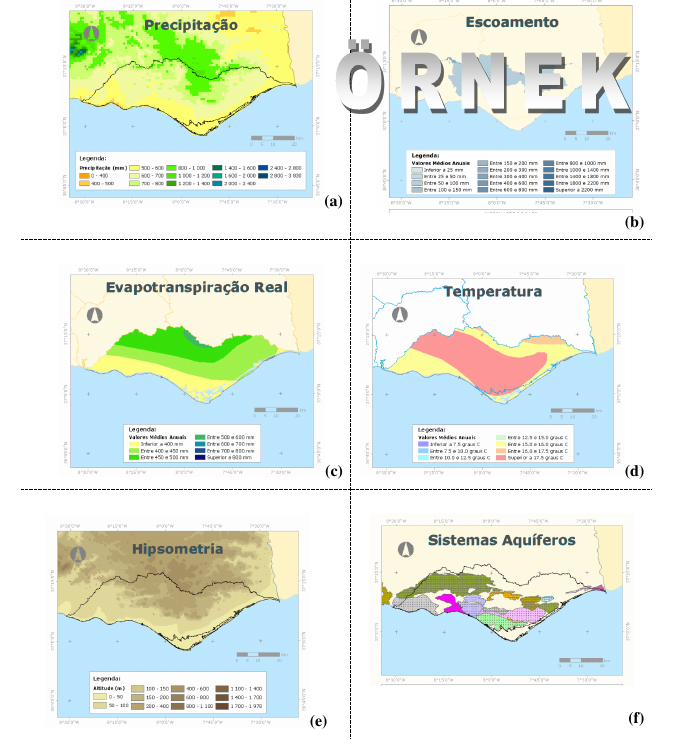
\includegraphics[width=430pt]{fig/haritalar} \caption{\label{fig:6-1}Bölgesel haritalar: (a)Yağış. (b)Akım. (c)Evapotranspirasyon
...}
\end{figure}

\noindent 
\begin{table}
\caption{\label{tableappendix2}Ekler bölümünde çizelge örneği.}

\centering{}%
\begin{tabular}{cccc}
\hline 
Kolon A  & Kolon B  & Kolon C  & Kolon D \tabularnewline
\hline 
Satır A  & Satır A  & Satır A  & Satır A \tabularnewline
Satır B  & Satır B  & Satır B  & Satır B \tabularnewline
Satır C  & Satır C  & Satır C  & Satır C \tabularnewline
\hline 
\end{tabular}
\end{table}

Lorem ipsum dolor sit amet, consectetur adipiscing elit. Sed ac augue
vel dui adipiscing placerat et nec metus. Donec bibendum sodales mollis.
Cras in lacus justo, at vestibulum quam. Sed semper, est sit amet
consectetur ornare, leo est lacinia velit, adipiscing elementum lectus
felis at sem.

\newpage{}

\chapter{EK A.2: Diğer Haritalar}

Lorem ipsum dolor sit amet, consectetur adipiscing elit. Sed ac augue
vel dui adipiscing placerat et nec metus. Donec bibendum sodales mollis.
Cras in lacus justo, at vestibulum quam. Sed semper, est sit amet
consectetur ornare, leo est lacinia velit, adipiscing elementum lectus
felis at sem.

\noindent 
\begin{figure}[h!]
\centering{}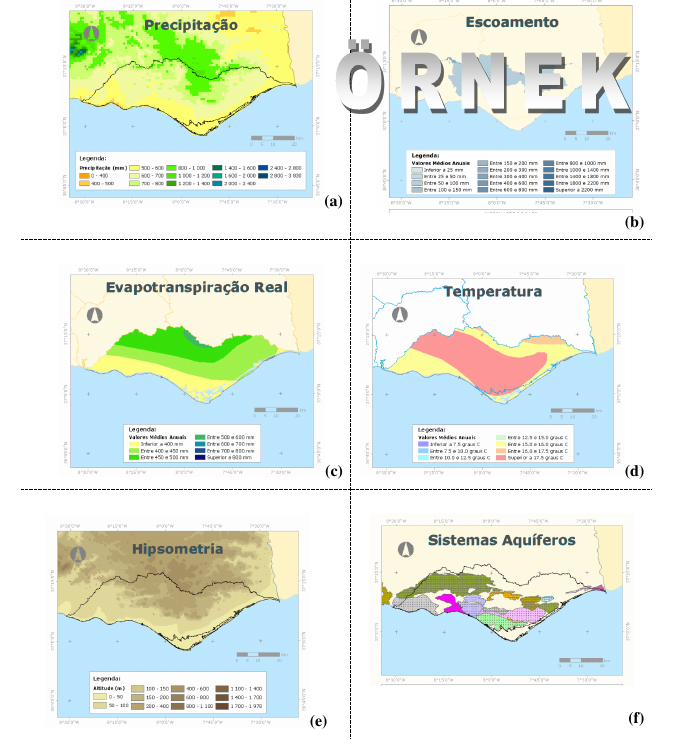
\includegraphics[width=430pt]{fig/haritalar} \caption{\label{fig:6-1-1}Bölgesel haritalar: (a)Yağış. (b)Akım. (c)Evapotranspirasyon
...}
\end{figure}

\noindent 
\begin{table*}[!ht]
\caption{\label{tableappendix2-1}Ekler bölümünde çizelge örneği.}

\centering{}%
\begin{tabular}{cccc}
\hline 
Kolon A & Kolon B & Kolon C & Kolon D\tabularnewline
\hline 
Satır A & Satır A & Satır A & Satır A\tabularnewline
Satır B & Satır B & Satır B & Satır B\tabularnewline
Satır C & Satır C & Satır C & Satır C\tabularnewline
\hline 
\end{tabular}
\end{table*}

Lorem ipsum dolor sit amet, consectetur adipiscing elit. Sed ac augue
vel dui adipiscing placerat et nec metus. Donec bibendum sodales mollis.
Cras in lacus justo, at vestibulum quam. Sed semper, est sit amet
consectetur ornare, leo est lacinia velit, adipiscing elementum lectus
felis at sem.

\newpage{}

\chapter{EK A.3: Diğer Diğer Haritalar}

Lorem ipsum dolor sit amet, consectetur adipiscing elit. Sed ac augue
vel dui adipiscing placerat et nec metus. Donec bibendum sodales mollis.
Cras in lacus justo, at vestibulum quam. Sed semper, est sit amet
consectetur ornare, leo est lacinia velit, adipiscing elementum lectus
felis at sem.

\noindent 
\begin{figure}[h!]
\centering{}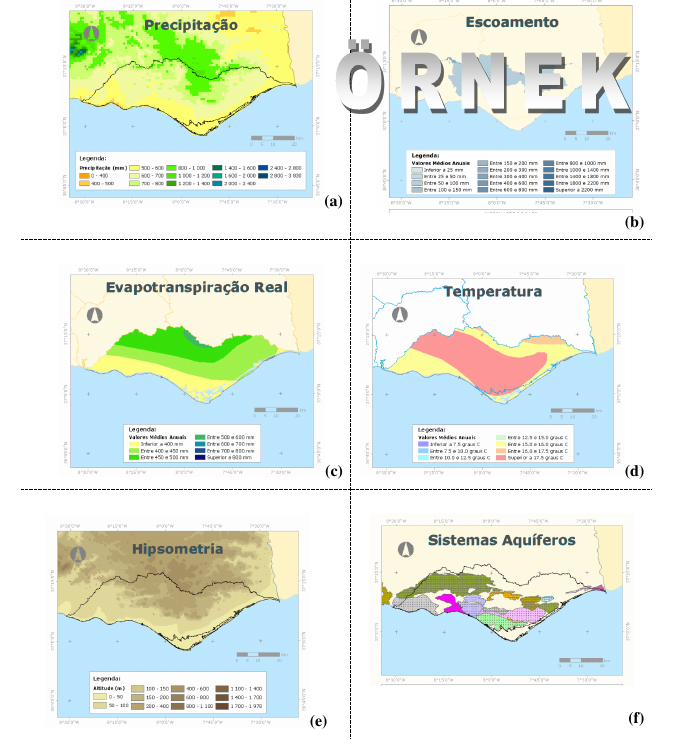
\includegraphics[width=430pt]{fig/haritalar} \caption{\label{fig:6-1-1-1}Bölgesel haritalar: (a)Yağış. (b)Akım. (c)Evapotranspirasyon
...}
\end{figure}

\noindent 
\begin{table*}[!ht]
\caption{\label{tableappendix2-1-1}Ekler bölümünde çizelge örneği.}

\centering{}%
\begin{tabular}{cccc}
\hline 
Kolon A & Kolon B & Kolon C & Kolon D\tabularnewline
\hline 
Satır A & Satır A & Satır A & Satır A\tabularnewline
Satır B & Satır B & Satır B & Satır B\tabularnewline
Satır C & Satır C & Satır C & Satır C\tabularnewline
\hline 
\end{tabular}
\end{table*}

Lorem ipsum dolor sit amet, consectetur adipiscing elit. Sed ac augue
vel dui adipiscing placerat et nec metus. Donec bibendum sodales mollis.
Cras in lacus justo, at vestibulum quam. Sed semper, est sit amet
consectetur ornare, leo est lacinia velit, adipiscing elementum lectus
felis at sem.

\newpage


\noindent \ozgecmis{\vspace{10mm}

\noindent %Bu bölüm resim koymak içindir. Resim koymak istemiyorsanız, resim dosyasının tanımlandığı satırın başına "%" işareti koyabilirsiniz.
%Resim koymak istiyorsanız, kendi resminizin dosyasını "CV.jpg" olarak kaydetmeniz yeterlidir ve bu bu bölümde herhangi bir değişiklik yapmanıza gerek yoktur.

\newsavebox{\mysquare}
\savebox{\mysquare}{\textcolor{black}{\rule[2.3pt]{3.4pt}{3.4pt}}}

\setlength{\TPHorizModule}{10pt}
\setlength{\TPVertModule}{10pt}

\begin{textblock}{1}(40,10)
 	\begin{figure}[p]
        % Resim dosyasını burada tanımlayın. Resim girilmesi zorunlu değildir.
		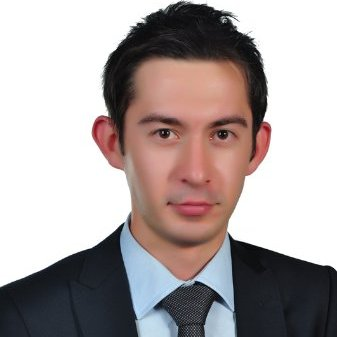
\includegraphics[width=3.5cm,keepaspectratio=true]{./fig/CV.jpg}
	\end{figure}
\end{textblock}

\noindent \textbf{Ad Soyad:} Ahmet Karabacak \\

\vspace{-3mm}
 \textbf{Doğum Tarihi ve Yeri:} 1993, Konya \\

\vspace{-3mm}
 \textbf{E-Posta:} ahmet7k@gmail.com \\

\textbf{ÖĞRENİM DURUMU:} \vspace{-3mm}

\begin{itemize}
\item \textbf{Lise:} 2011, Konya Atatürk Lisesi 
\item \textbf{Lisans:} 2016, Eskişehir Osmangazi Üniversitesi, İnşaat Mühendisliği 
\item \textbf{Y. Lisans:} 2019, İstanbul Teknik Üniversitesi, Deprem Mühendisliği
\end{itemize}
\textbf{MESLEKİ DENEYİMLER VE ÖDÜLLER:} \vspace{-3mm}

\begin{itemize}
\item Soyut İnşaat 2013-2016 ,Yarı-zamanlı mühendislik uygulamaları
\item 2014-2016 tarihlerinde Eskişehir Osmangazi Üniversitesi İnşaat Mühendisliği
Bölüm Temsilciliği
\item 2014 yılında TAV İnşaat Emaar Square Projesinde saha stajı
\item 2015 yılında Alarko Holding merkez ofis, arazi değerlendirme departmanında
ofis stajı
\item Erdemli Proje Müşavirlik 2016- Halen , Yapı Tasarım Mühendisi
\item Bu tez 42127 numaralı İTÜ Bilimsel Araştırma Projesi kapsamında kabul
edilmiştir.
\end{itemize}
% ---------------------------------------------------------------- %
% Fotografli ve yayin listeli (yayini varsa) ozgecmis onerilir.    %
% Fotograf ve adres sart degildir.                                 %
% -----------------------------------------------------------------%
}
\end{document}
